%%%%%%%%%%%%%%%%%%%%%%%%%%%%%%%%%%%%%%%%%%%%%%%%%%%%%%%%%%%%%%%%%%%%%%%%%%%%%%%
%%%%%%%%%%%%%%%%%%%%%%%%%%%%%%%%%%% PREAMBLE %%%%%%%%%%%%%%%%%%%%%%%%%%%%%%%%%%
%%%%%%%%%%%%%%%%%%%%%%%%%%%%%%%%%%%%%%%%%%%%%%%%%%%%%%%%%%%%%%%%%%%%%%%%%%%%%%%

\documentclass[12pt, a4paper]{article}

\usepackage[top=2.5cm, bottom=2.5cm]{geometry}

\usepackage[utf8]{inputenc}
\usepackage[backend=bibtex, style=nature]{biblatex}
\usepackage{color,soul}
\usepackage{amsmath}
\usepackage[T1]{fontenc}
\usepackage{graphicx}
\usepackage{caption}
\usepackage{xargs}                      		% Use more than one optional parameter in a new commands
\usepackage[pdftex,dvipsnames]{xcolor}  		% Coloured text etc.
\usepackage{booktabs}   					% table formatting
\usepackage{textcomp}
\usepackage{siunitx}
\usepackage{rotating}    					% sideways figure environment
\usepackage{adjustbox}    					% sideways figure environment
\usepackage{setspace}
\usepackage{float}
\usepackage{authblk}
\usepackage[nottoc]{tocbibind}
\usepackage{placeins}

\usepackage[singlelinecheck=false]{caption}

%todonotes customisation
\usepackage[colorinlistoftodos,prependcaption,textsize=tiny]{todonotes}

\captionsetup[figure]{labelfont={bf},labelformat={default},labelsep=period,name={Supplementary Figure}}

\captionsetup[table]{labelfont={bf},labelformat={default},labelsep=period,name={Supplementary Table}}

\addbibresource{papers_library} 

\usepackage[unicode]{hyperref}

\renewcommand{\listfigurename}{Supplementary Figures}
 
\renewcommand{\listtablename}{Supplementary Tables}

\renewcommand\Affilfont{\fontsize{8}}

%%%%%%%%%%%%%%%%%%%%%%%%%%%%%%%%%%%%%%%%%%%%%%%%%%%%%%%%%%%%%%%%%%%%%%%%%%%%%%%%%%%
%%%%%%%%%%%%%%%%%%%%%%%%%%%%%%%%%%% FRONT MATTER %%%%%%%%%%%%%%%%%%%%%%%%%%%%%%%%%%
%%%%%%%%%%%%%%%%%%%%%%%%%%%%%%%%%%%%%%%%%%%%%%%%%%%%%%%%%%%%%%%%%%%%%%%%%%%%%%%%%%%

\title{\textbf{Social tipping points in global groundwater management}}
\author[1,*]{Juan Carlos Castilla-Rho}
\author[2]{Rodrigo Rojas}
\author[5,4]{Cameron Holley}
\author[3,4]{Martin Andersen}
\author[6]{Gregoire Mariethoz}

\affil[1]{CSIRO Land and Water, Perth WA 6014, Australia}
\affil[2]{CSIRO Land and Water, Brisbane QLD 4102, Australia}
\affil[3]{UNSW, School of Civil and Environmental Engineering, Sydney NSW 2052, Australia}
\affil[4]{Connected Waters Initiative Research Centre, Sydney NSW 2052, Australia}
\affil[5]{UNSW, Faculty of Law, Sydney NSW 2052, Australia}
\affil[6]{Institute of Earth Surface Dynamics, University of Lausanne, Switzerland}
\affil[*]{Corresponding author, Juan.Castilla@csiro.au}

\date{}                     %% if you don't need date to appear
\setcounter{Maxaffil}{0}
\renewcommand\Affilfont{\itshape\small}

%%%%%%%%%%%%%%%%%%%%%%%%%%%%%%%%%%%%%%%%%%%%%%%%%%%%%%%%%%%%%%%%%%%%%%%%%%%%%%%%%%%
%%%%%%%%%%%%%%%%%%%%%%%%%%%%%%%%%%% DOCUMENT %%%%%%%%%%%%%%%%%%%%%%%%%%%%%%%%%%%%%%
%%%%%%%%%%%%%%%%%%%%%%%%%%%%%%%%%%%%%%%%%%%%%%%%%%%%%%%%%%%%%%%%%%%%%%%%%%%%%%%%%%%

\begin{document}

\maketitle

\tableofcontents

\newpage

\listoffigures
\listoftables

\setcounter{secnumdepth}{0}

\onehalfspacing

\section{Supplementary Discussion} \label{SI Discussion}

\subsection{Cultural Theory: Background and Justification}

Cultural Theory \autocite{Douglas:2004um} (also referred to as Grid-Group or Plural Rationality Theory) conceptualises human behaviour according to four broad types of social organisation, or ‘ways of life’, (hierarchist, individualist, fatalist and egalitarian) co-existing with different degrees of dominance in every society. The theory postulates that people are especially concerned with two aspects of social life: Grid and Group. Grid represents reliance on standards (e.g., customs, morals, shame) for achieving goals. Low grid people have a desire for nonconformity and a belief that nonconformist behaviour leads to individual success. High grid people rigidly adhere to social norms and they are more willing to punish actions that violate these norms, even if this generates no direct benefits to them \autocite{Henrich:2006gj, Chai:2009vz}. Group represents how strongly people in a society are bonded together. Low-group people are self-focused and competitive; high-group people have interests that overlap with the interests of the collective. Together, grid and group form a two-dimensional representation of cultural types, split into quadrants that define four general typologies of human behaviour or ‘ways of life’: individualist, egalitarian, fatalist, and hierarchist (see main text Figure 1). 

Cultural Theory has become the topic of a lively debate between proponents and critics of the approach. The criticism evolves around whether the theory captures historical circumstances, where the Grid and Group concepts come from, and at what level it should be applied (for an in depth discussion see \autocite{Verweij:2000tx}). By far, the most common critique on Cultural Theory is that it is based on ‘just’ four categories, and that this simplicity overlooks the great variety of alternative ways of living and perceiving. Verweij et al.\autocite{Verweij:2000tx} and Rotmans and de Vries \autocite{Rotmans:1997td} argue in favour of this simplicity, noting that: (1) the four categories provide a systematic and coherent taxonomy of the ways in which actors perceive and construct all kinds of international issues; (2) the four categories enable researchers to condense the multitude of ideas, values, perceptions, and beliefs of agents into a limited, manageable set of rationalities; and (3) it makes different cases comparable.

Cultural Theory has been employed in the fields of anthropology, sociology, political science and public administration \autocite{Verweij:2000tx}. Its main appeal is that it offers a straightforward typology for the analysis of social processes and a basis for testing general statements about how people think and act \autocite{Verweij:2015cr}. In this study, we chose to use the framework of Cultural Theory because of the need to compare social contexts. Cultural Theory has been applied, for example, to the study of transboundary water resources (e.g., the Rhine River and the American Great Lakes) \autocite{Verweij:2000tx}, preferences and risks of water reuse \autocite{Hoekstra:2000il}, and sustainable water resource management \autocite{Offermans:2011ja}. O'Riordan and Jordan \autocite{ORiordan:1999ko} recommend Cultural Theory for explaining patterns of thinking that shape communication, information gathering and interpretive aspects of climate change politics and science. Caulkins and Peters \autocite{Caulkins:1999fz} argue that the grid-group concept has been successfully applied by an interdisciplinary group of scholars to help explore environmentalist views. Rotmans and de Vries \autocite{Rotmans:1997td} use Cultural Theory to characterise the broad spectrum of people’s worldviews in relation to socio-environmental systems and sustainability (with some differences: fatalists are excluded from their framework of perspectives). Verweij et al.\autocite{Verweij:2015cr} contend that the most influential social theories of the last four decades—rational choice theory, behavioural economics, and post-structuralism—contain assumptions that are inconsistent with key findings in affective and social neuroscience, but they are in line with Cultural Theory. For an in-depth discussion about the motivations for using Cultural Theory in sustainability science, see \autocite{Rotmans:1997td}.


\section{Supplementary Methods} \label{SI Methods}


\subsection{Obtaining Grid and Group scores from the World Values Survey Wave 6 (2010-2014)}

Currently there is no large-scale survey that directly measures grid and group characteristics of people. In order to measure the grid and group dimensions, one must carry out secondary analyses, that is, process data that was not originally designed to compute grid and group scores \autocite{Chai:2009vz, Grendstad:1999cp}. Such data may be found in large scale surveys covering a large number of topics, such as the World Values Survey (WVS; \url{https://www.worldvaluessurvey.org}). The WVS is conducted through detailed questionnaires in face-to-face interviews. Questionnaires for the WVS6 (2010-2014) consist of 258 questions administered to about 1,000 to 3,500 interviewees per country, with a worldwide total of 90,350 interviews. 

For consistency, qualitative validation and to allow comparisons, we applied the methodology proposed by Chai et al. \autocite{Chai:2009vz} to compute for the first time, to our knowledge, grid and group indices for the 57 countries covered by the WVS6 (main text Figure 1, Supplementary Figure \ref{Fig: CH3_GCGP1_WVS raw stats all countries boxplots}). The process of determine grid and group positions from the WVS developed by Chai et al. is as follows:

\begin{itemize}

\item Discard questions that are not pertinent to either grid or group. Questions regarding specific political parties and issues are eliminated since they are pertinent only to a specific geographic location and political system. However, general questions of a political nature, such as those regarding the proper role of government in the economy, were not excluded. Finally, although questions about happiness and life satisfaction could conceivably be correlated with positions on the grid or group dimensions, such questions are likely to rest on emotional states in a manner that may be different from questions that represent more straightforward beliefs and values about the larger world. Thus, these questions also are also excluded. The net effect of the previously mentioned review process through a grid-group lens means that 59 questions are retained. \item Isolate those questions that carry the most useful information about the Grid and Group dimensions. The list of 59 questions is further reduced to 10 grid questions and 10 group questions, chosen because they exhibit the highest variations across countries i.e., those with the highest F-statistic, from a one-way analysis of variance (ANOVA). Supplementary Table \ref{table: WVS grid-group questions}, shows that computed grid and group scores for the selected questions exhibit significantly less variance within societies than between societies (P<0.001), meaning that these indices provide sufficiently large variation to highlight differences between countries. The aim of this step is to use the smallest number of questions that give the largest payoff in explanatory power. Moreover, the 20 questions chosen cover a wide range of topics (see Supplementary Table \ref{table: WVS grid-group questions}); this offers an unbiased and fair sample of questions to generate our indices. Although we could add more questions, they do not provide statistically significant additional information about differences in grid-group positions between countries. \item Normalise answers to each question onto a scale of 0 to 1. This avoids the inconsistent scaling and scoring of answers for different questions in the WVS. \item Average the scores for the questions under each social dimension to generate final grid and group scores. Scores are computed using equal weights because there is no theoretically informed a priori reason to assign one question greater importance than another in determining grid or group positions. Equal weighting is the most parsimonious approach and is commonly applied in social research \autocite{Babbie:2010vh} as this avoids introducing weight coefficients without clear justification. Even weighting is also used in a number of well-known social indexes, such as the Happy Planet Index (\url{http://happyplanetindex.org}) and the Human Development Index (\url{http://hdr.undp.org/en}).
\end{itemize}

Supplementary Table \ref{table: WVS grid-group questions} categorises the grid (10) and group (10) questions that were used to calculate grid-group scores. Grid questions represent opinions about the individuation of members of the organisation and the degree to which their choices are constrained by imposed rules and role descriptions. High grid refers to a social environment where individual interactions are regulated and autonomy is minimal. Group questions represent opinions about the value people place on relationships with the collective and the commitment they have to the larger social unit. High group refers to a social environment where people value collective relationships and commit to the larger social unit. Supplementary Figure \ref{Fig: CH3_GCGP1_WVS raw stats all countries boxplots} presents a summary of raw statistics for grid and group scores.

It is important to clarify that the four categories proposed by Cultural Theory (fatalist, individualist, egalitarian, hierarchist) are simply heuristics that are meant to illuminate culture patterns at an aggregate level. These cultural groups are not clearly bounded sets for which a single label can be placed, but may encompass characteristics of multiple cultures that further exhibit internal variation. This is why in Supplementary Figure \ref{Fig: CH3_GCGP1_WVS raw stats all countries boxplots} we report summary statistics for grid and group scores.

To derive Figure 1 (main text), we normalised the data presented in Supplementary Figure \ref{Fig: CH3_GCGP1_WVS raw stats all countries boxplots} by the minimum and maximum grid and group country average scores. The reason is to allow for consistent parametrisation of agents in the GCG, whose grid and group parameters are allowed to vary between 0 and 1. Grid and group scores were used to evaluate the functional form of social utility (S) of our GCG agents. S combines the effects of two social concerns: (1) the social costs of reporting non-compliant neighbours (i.e., the burden of being the whistle-blower), and (2) the social costs of developing a bad reputation when caught breaking the rules. For details, see ODD+D model documentation below.

\subsection{Validation of Grid-Group positions}

Grid-Group positions shown in Figure 1 (main text) correspond to what one would expect from the ethnographic literature. The following correlations are consistent with the analysis of the WVS3 and WVS4 of Chai et al.\autocite{Chai:2009vz}:

\begin{enumerate}
	\item \textbf{Socioeconomic correlation} is observed between countries with similar cultural characteristics e.g., most developed countries have lower grid values than developing countries (see Supplementary Figure \ref{Fig: CH3_GCGP1_WVS raw stats all countries boxplots}a).
	\item \textbf{Geographical correlation.}  For example, New Zealand and Australia, which are geographically adjacent as well as former British colonies, both belong to the egalitarian category (a similar observation can be made for Argentina and Uruguay). Eastern European countries such as Romania, Russia, Poland, Belarus, Turkey and Ukraine are close to each other, and are located within the high-grid and low-group quadrant, implying that these are relatively fatalist. African countries like Ghana, Zimbabwe, Nigeria, Tunisia and Algeria are also close to each other, and classify under the fatalist category.
	\item \textbf{Ethnicity and religion} play a very important role in the variation of grid and group characteristics. For instance, newly independent countries and Muslim countries exhibit similar group scores. Our results show that predominantly middle eastern countries tend to have higher grid and group than other countries.
\end{enumerate}

\subsection{Validation of the WVS and GCG results: Murray-Darling Basin surveys}

Grid group indicators derived from the WVS were statistically tested against data from our empirical surveys in the Murray-Darling Basin dataset. We have shown that the WVS is consistent with grid-group positions of farmers in rural Australia to a statistically significant level (see below). We note that surveys with a sample size like the one we have obtained in the Murray-Darling Basin are uncommon; they also require significant time and financial resources to collect. Thus, concerted efforts are required to conduct similar validation in other regions. 

To test the validity of the GCG in a real-world groundwater management scenario, we computed indices for grid group (see Supplementary Table \ref{table: MDB grid-group questions}), monitoring (M), fines (F), and compliance from a quantitative survey of approximately 4000 water license holders (22\% response rate) conducted by the authors between September 2012 and January 2013 in New South Wales, eastern Australia \autocite{Holley:2015te}. The survey captured water users’ views on compliance motivations, experiences with compliance and enforcement by the New South Wales Office of Water, water users’ information sources, and their knowledge of water regulation. 

Grid and group indices computed from the New South Wales survey surveys do not differ significantly from indices obtained from the WVS6 (parametric t-test; nWVS=1477 and nMDBsurvey=672; two-sided P=0.12 for grid and P=0.65 for group). Empirical values for monitoring (M), fines (F), and compliance were obtained from survey questions ‘q2off’ (“compliance officers from the New South Wales Office of Water work regularly in my region”) and ‘q3pro’ (“people illegally taking water will be prosecuted”), ‘q3det’ (“the penalties for illegal water extraction are a strong deterrent”) and ‘q3crim’ (“getting a criminal record for carrying out illegal water activities is a strong deterrent”), and ‘q3big’ (“illegal water extraction is a big problem in my region”), respectively. Observed compliance was consistent with our simulations (see Supplementary Figure \ref{fig: CH3_GCG1_WVS-MDB validation}).

\subsection{Murray-Darling Basin surveys: sample collection}

There are a large number of water users in New South Wales (NSW). As of June 2011, there were over 7000 surface water licences and 71,000 groundwater (bore) licences managed under the Water Act 1912 (NSW) and over 24,000 surface and groundwater licences under the Water Management Act 2000 (NSW).  As of 30 June 2011, 58 per cent of Water Act 1912 (NSW) licences had been converted to tradable Water Access Licences under the Water Management Act 2000 (NSW). These water users draw on a diversity of water sources (unregulated surface water, regulated surface water and groundwater) for a variety of purposes (e.g. stock and domestic and irrigation). Furthermore, water users themselves vary greatly in terms of property size, land use (e.g. grazing, horticulture), and other characteristics (e.g. membership of irrigation schemes, industry associations, water user groups). Given this diversity, it was decided that a quantitative survey was the best approach to try and capture relevant data. The survey was conducted in three catchments/regions:

\begin{enumerate}
	\item Macquarie-Bogan in the Central West (CW).
	\item Murrumbidgee/Murray Riverina in the Murray and Murrumbidgee (MM).
	\item Richmond in the North Coast (NC). 
\end{enumerate}

These regions were selected purposively to represent a diversity of:

\begin{enumerate}
	\item Water sources (regulated rivers, unregulated rivers and groundwater).
	\item Locations (MM and CW are both inland, while NC is coastal).
	\item Authorisations (e.g. licences, approvals and stock and domestic).
	\item ‘At risk’ water sources as defined for the National Framework for Compliance and Enforcement Systems for Water Resource Management.  
\end{enumerate}
 
Across all three regions smaller stock and domestic water users were also included. Taking water under a basic landholder right has historically been subject to little oversight by regulatory agencies. For example, water taken for stock and domestic use is not required to be metered. While such uses have a minimal impact individually on overall water consumption, they may cumulatively have a much more significant impact (with 100,000s of stock and domestic water users across the state).

Taking into consideration resource and practical constraints, the survey began with a raw list of 4500 licence and approval holders (approximately 1500 from each of the three regions, chosen to include a full range of water users from large entitlement holders extracting water for commercial use to people extracting water solely for stock and domestic purposes). The list was refined to create a more targeted survey list, including ensuring multiple works/licence holders would only receive one survey and removal of any repeat or incomplete addresses, as well as entries pertaining to local/state governments and commercial companies outside of NSW (who were unlikely to have the desired knowledge and experience with on property water use). A final survey list was sent to 1381 CW, 1258 MM and 1339 NC properties (totalling 3,978). The survey numbers and response rates are summarised in \autocite{Holley:2015te}.

In terms of the data gathered being representative, there may be differences between respondents and non-respondents to mail surveys such as the one conducted in the Murray Darling Basin.  Statistical comparisons of the property and social background data could not be made because the area covered by Australian Bureau of Statistics statistics does not match the surveyed areas and sourced population.  While a lower response increases the likelihood that non-respondents to the survey are significantly different to respondents, response rates by themselves are not good indicators of non-respondent bias, and it is impossible to completely correct for all non-respondent bias.


%%%%%%%%%%%%%%%%%%%%%%%%%%%%%%%%%%%%%%%%%%
%%%%%%% ODD+D MODEL DOCUMENTATION %%%%%%%%
%%%%%%%%%%%%%%%%%%%%%%%%%%%%%%%%%%%%%%%%%%
  
\subsection{ODD+D Model Documentation}

Grimm et al.\autocite{Grimm:2006it} have proposed a standard protocol termed ODD (Overview, Design concepts, and Details) aimed at the description of agent-based models in ecology, with a view to its application in agent-based social simulation and other disciplines. ODD is designed to ensure that such descriptions are readable and complete. ODD is intended to facilitate readability through stipulating a structure for the description with a logical ordering. The structure also contains guidelines for the contents of the description, designed to ensure that all relevant information about a model is captured, at least for the purposes of understanding the application in the associated article, and for replication. Müller et al.\autocite{Muller:2013dk} have recently extended ODD to ODD+D so that it is easier to have a standard way of describing human decision-making within agent-based models.

We answer the guiding questions that should be answered by the model description and to give a precise description of the Groundwater Commons Game. This will give readers of the description a better understanding of the simulated decision-making process.

\subsubsection{ODD+D: Overview}

The overview section consists of the subsections i) purpose, ii) state variables and scales, and iii) process overview and scheduling.

\paragraph{I.i Purpose }

\paragraph{I.i.a What is the purpose of the study?}

To synthesise and extend existing work on human cooperation and collective action, to elucidate possible determinants and pathways to regulatory compliance in groundwater systems globally. We have designed the `Groundwater Commons Game' (GCG) as a scientific instrument to systematically investigate mechanisms that may lead to compliance with groundwater conservation policies, taking into consideration human behavioural variables revealed by the World Values Survey. The study aims to:

\begin{itemize} \item offer general insights that are applicable to aquifers everywhere \item parametrise agent behaviours using the most recent version of the World Values Survey \item develop GCG simulations for three real-world case studies; the Punjab (India/Pakistan), the Central Valley (USA), and the Murray-Darling Basin (Australia) \item assess the validity of results using surveys from the Murray-Darling Basin \item propose policy recommendations of global relevance \end{itemize}

More broadly, the systems understanding that we present here has general implications to any regulated resource that is accessed by many users, as in the case of fisheries, forests, wildlife and global climate.

\paragraph{I.i.b For whom is the model designed?}

The model is designed for groundwater scientists, groundwater managers, decision and policy makers interested in natural resource management and regulatory compliance. The GCG can also be used for learning activities in undergraduate and graduate courses in environmental management.

Water managers typically evaluate the performance of enforcement and compliance policies via manager experiences, outcomes from enforcement actions, field surveys and interviews. These instruments however may not reveal the true motivations and attitudes towards water regulation. The cost and time of conducting empirical research can be significant. These are major challenges for decision-makers searching for courses of action that lead to long-term compliance and extend economic activity in groundwater basins subject to depletion. Simulation-based approaches like the one proposed here can help water authorities overcome the difficulties of studying rule-breaking behaviour directly, and provide new insights on how human behaviour impacts resource conservation at the global scale.

\paragraph{I.ii Entities, state variables, and scales}

\paragraph{I.ii.a What kinds of entities are in the model?}

\begin{itemize} \item Individual farmers \item A water authority/regulator \item The groundwater resource---a physical entity \item The agricultural region---defined by the number of farmers and the local economy \end{itemize}

\paragraph{I.ii.b By what attributes (i.e. state variables and parameters) are these entitiescharacterized?}

\textbf{Farmer:} geographical location (determines depth to water table), irrigated acreage [ha], gross margins from crop [\$/ha], behavioural strategy (B=boldness, P=punitiveness), pumping decision (comply, defect), mutation probability (probability that the agent will try a new strategy, fixed at 5\%), Economic utility (E), Institutional utility (I), Social utility (S), overall Performance Index (PI=E*I*S), rule-follower (yes/no), grid/group scores (determined from the WVS, see Methods), pump efficiency (\textasciitilde{}80\% for centrifugal pumps), returns [\$/ha], irrigated area [ha].

\textbf{Water authority:} Pumping cap (\% of licensed allocations), \% monitoring capacity (M, 0-50\%), magnitude of monetary fines (F, representing the fraction of farmer profit forgone to pay a fine), risk-based management (yes/no), monitoring style (constant/adaptive), graduated sanctions (yes/no).

\textbf{Groundwater:} model size [km\textsuperscript{2}], number of cells, cell dimensions [m], boundary conditions (no-flow, specified-flux), aquifer thickness [m], hydraulic conductivity [m/d], storativity, initial heads [m].

\textbf{Agricultural region:} number of farmers per [ha], crop parameters (type, price [\$/ton], yield [ton/ha], water requirement [ML/ha], energy price [\$/kWh], other variable costs [\$/ha])

\paragraph{I.ii.c What are the exogenous factors / drivers of the model?}

\begin{itemize} \item Country-level Grid-Group scores determined from the World Values Survey \item Level of monitoring (M) and fines (F) adopted by the water authority \item \% rule-followers in the population \item Groundwater conditions (hydraulic parameters, boundary conditions) \end{itemize}

\paragraph{I.ii.d If applicable, how is space included in the model?}

Explicitly through the location of each farm within the modelled domain. The depth to groundwater is spatially variable (following the hydraulics of groundwater flow), thus location determines the costs to extract groundwater, and the information each farmer has on his/her neighbour's strategies.

\paragraph{I.ii.e What are the temporal and spatial resolutions and extents of the model?}

Six-month timesteps over a period of 100 years. The first 50 years represent a burn-in period without management, followed by 50 years of groundwater regulation. Irrigation decisions are taken at the beginning of a season, i.e. once a year, except in the wheat-rice rotation in Punjab example where irrigation decisions are taken twice a year.

The groundwater sub model represents a 10x10 [km] basin, discretised into 40x40 cells. The dimension of each cell is 200 [m]. Model boundary conditions are defined by a no-flow boundary to the North and South, and constant head boundary cells to the East and West; setting head values to create an East-West gradient of 1/1,000 representing typical conditions in regional aquifer systems. Groundwater is pumped from a semi-confined sand aquifer of 50 m thickness, hydraulic conductivity K=10 [m/d] and storativity S=10\textsuperscript{-4}.

\subsubsection{ODD+D: Design Concepts}

In this section, we describe ten design concepts based on the ODD+D protocol. There is a gradient from the overall view (the theoretical and empirical background, individual decision-making and learning) to the details (e.g. individual sensing and prediction). The stochasticity and observation relate to more technical questions are placed at the end of the section.

\paragraph{I.iii Process overview and scheduling}

\paragraph{I.iii.a What entity does what, and in what order?}

See Supplementary Figure \ref{Fig: CH3_GCG1_Flow diagram agent processes}

\paragraph{II.i Theoretical and Empirical Background}

\paragraph{II.i.a Which general concepts, theories or hypotheses are underlying the model's design at the system level or at the level(s) of the sub model(s) (apart from the decision model)? What is the link to complexity and the purpose of the model?}

Tipping points and critical transitions \autocite{Scheffer:2012ct, Scheffer:2001ij,Scheffer:2009gg}, theory of complexity and complex adaptive systems \autocite{Miller:2009uu}, groundwater hydraulics \autocite{Fetter:2001tx}. The link to complexity related to emergent patterns across the grid-group plane in the form of tipping points. This suggests that certain social interactions and nonlinearities in the system can be exploited to trigger long-term resource conservation.

\paragraph{II.i.b On what assumptions is/are the agents' decision model(s) based?}

Agents are bounded rational \autocite{Simon:1955bf}, use a form of inductive reasoning \autocite{Deadman:to}, rely on heuristics \autocite{Ostrom:1994ti} and they have no foresight \autocite{Gigerenzer:2007wy, Gigerenzer:2002tn}.

Agents engage in a process of trial and error to determine their best decision (how to update their strategies in terms of B and P) based on their experience with past strategies and the imitation of successful neighbours. This assumption is supported by recent work in the context of the role of imitation in land use change and the adoption of agricultural innovations, and work on imitation in spatial games \autocite{Gotts:2009td}—this research confirms that farmers are influenced toward adopting new land uses, techniques, or behaviours by the example of other farmers they know. Studies of the spatial characteristics of innovation diffusion also indicate that imitation of neighbours is important.

\paragraph{II.i.c Why is a/are certain decision model(s) chosen?}

The decision model of the water authority is based on real-world attributes of groundwater governance systems.

The decision model of farmers builds on Robert Axelrod's seminal paper on the emergence of social norms \autocite{Axelrod:1986vx}. Here, we adapt Axelrod's framework to study social norms in the context of compliance with groundwater conservation policies. The GCG is designed to be very general and the approach can be applied to any number of problems involving stressed groundwater systems. The structure and assumptions of the GCG can be easily tailored and/or extended to suit specific economic, institutional, social, and hydrogeological contexts.

Key changes to Axelrod's original model are:

\begin{enumerate} \def\labelenumi{\arabic{enumi}.} \item We consider local interactions between neighbouring agents, instead of a "soup" model as in Axelrod's model, where all agents interact with each other. In our model, monitoring and punishment is local instead of global; see \autocite{Gotts:2009td}. \item We incorporate the physics of groundwater flow as one of the drivers of agent behaviour. We explicitly quantify the economic damage (externality) imposed by defecting wells on other wells, which manifests as additional pumping costs incurred within a neighbourhood of the defecting well. The extent of this neighbourhood is determined by the local hydrogeological conditions and the magnitude of a breach. \item We use a combined score metric to quantify `fitness' of an agent at every moment, based on economic, institutional and social factors. In the Axelrod case, fitness is entirely driven by the social component. \item We introduce variability in the magnitude of breaches, as we would expect in agricultural settings. \item Breaches are not only enforced by agents, but also by a water authority: the water authority. Enforcement therefore occurs at the local and basin scales. \end{enumerate}

\paragraph{II.i.d If the model / a submodel (e.g. the decision model) is based on empirical data, where does the data come from?}

Agent behaviour is parametrised using Grid-Group dimensions obtained from Wave 6 of the World Values Survey.

The hydraulic properties of the groundwater sub model are typical of groundwater basins in alluvial settings \autocite{Margat:2013ty}. All hydrogeological parameters can be changed with frugal user intervention via the provided interface.

\paragraph{II.i.e At which level of aggregation were the data available?}

The WVS is conducted at the country-level and each wave represents a period of approximately four years.

\paragraph{II.ii Individual Decision Making}

\paragraph{II.ii.a What are the subjects and objects of decision-making? On which level of aggregation is decision-making modelled? Are multiple levels of decision making included?}

Decision making is modelled at two levels:

\begin{itemize} \item The water authority decides about the cap on groundwater allocations, the level of monitoring and the severity of fines \item The farmers decide about whether to comply with the allocations or not, and in doing so, the area of land that will be irrigated in a given year. \end{itemize}

\paragraph{II.ii.b What is the basic rationality behind agents' decision-making in the model? Do agents pursue an explicit objective or have other success criteria?}

Agents are assumed to employ a simple utility function to evaluate the social and economic implications of their actions. This utility function combines: an economic score (\emph{E}) that quantifies the gross margins of crop production, considering pumping costs based on local groundwater drawdowns; an institutional score (\emph{I}) that notionally represents the proportion (0-100\%) of gross margins forgone to pay fines; and a social score (\emph{S}) that notionally represents the loss of reputation (proportional to Group) and the social costs of reporting offenders (inversely proportional to Grid). These components are combined into an overall performance index \emph{PI}=\emph{E}*\emph{I}*\emph{S}, which agents use to compare and decide among competing strategies (B,P).

\paragraph{II.ii.c How do agents make their decisions?}

Agents rely on local information and operate on a simple heuristic to decide what do next: ``\emph{imitate} the strategy of whichever neighbour is doing best, \emph{exploit} the current strategy if better, and \emph{explore} a new strategy occasionally'' \autocite{Gigerenzer:2002tn}. Decisions that are selected on the criterion of their recent performance within the neighbourhood of the land parcel concerned---as implemented in our model---is known as "Best-mean Imitation". Gotts et al. \autocite{Gotts:2009td} show that Best-mean imitation outperforms other forms of imitation in a wide range of settings.

\paragraph{II.ii.d Do the agents adapt their behaviour to changing endogenous and exogenous state variables? And if yes, how?}

Yes, they use the imitation heuristic described above to adapt their behavioural strategies (B,P), which in turn define whether or not they will comply with water allocations and whether they will report offending neighbours.

\paragraph{II.ii.e Do social norms or cultural values play a role in the decision-making process?}

Indeed, our model focuses on a limited set of contextual factors that play a role in achieving community compliance---conservation policies, social norms, and cultural values. These factors have been identified as fundamental drivers of human cooperation \autocite{Nowak:2012hj, Axelrod:1997ug} and collective action \autocite{Ostrom:1990ws, Ostrom:1999gn, Dietz:2003tp} in a wide range of settings. Cultural parameters are derived from the World Values Survey (see Methods).

\paragraph{II.ii.f Do spatial aspects play a role in the decision process?}

Yes because the imitation of neighbours and the drawdown propagation are spatial factors influencing decisions.

\paragraph{II.ii.g Do temporal aspects play a role in the decision process?}

In this study we assume that agents have no memory of past decisions; however this feature is implemented in the model (see Netlogo version of the model in Open ABM repository).

\paragraph{II.ii.h To which extent and how is uncertainty included in the agents' decision rules?}

Uncertainty is incorporated as agents are only aware of information about their immediate neighbourhood and not those further afield. Another source of uncertainty is the strategy mutation rate (fixed at 5\%) which determines how often agent will choose to try a completely new strategy. This introduces novelty to the pool of strategies in the agent population.

\paragraph{II.iii Learning}

\paragraph{II.iii.a Is individual learning included in the decision process? How do individuals change their decision rules over time as consequence of their experience?}

Learning occurs via a "best-mean imitation" heuristic \autocite{Gotts:2009td} based on past performance of strategies within the neighbourhood of the land parcel concerned. The heuristic is: \emph{imitate} the strategy of whichever neighbour is doing best, \emph{exploit} the current strategy if better, and \emph{explore} a new strategy occasionally'' \autocite{Gigerenzer:2002tn}.

\paragraph{II.iii.b Is collective learning implemented in the model?}

Collective learning is not implemented in the model but it is an emergent property of the system. The decision heuristic is a genetic algorithm which the agent population uses to discover and exploit decisions that provide the highest utility, considering the simultaneous decisions of the collective

\paragraph{II.iv Individual Sensing}

\paragraph{II.iv.a What endogenous and exogenous state variables are individuals assumed to sense and consider in their decisions? Is the sensing process erroneous?}

Individuals sense depth to water table, irrigation costs, yields and their budget. All these variables are known without error.

\paragraph{II.iv.b What state variables of which other individuals can an individual perceive? Is the sensing process erroneous?}

A farmer can perceive the Performance Index (PI) and strategy (B,P) of its immediate neighbours (i.e., we assume they can look over the fence).

The water authority can assess whether a farmer has complied or not with the allocated water, provided there is sufficient capacity and resources to send inspectors to the field (M determines the maximum number of farmers that can be audited in a given year)

All these parameters and behaviours are known without error.

\paragraph{II.iv.c What is the spatial scale of sensing?}

Basin (water authority), immediate neighbourhood (farmers).

\paragraph{II.iv.d Are the mechanisms by which agents obtain information modelled explicitly, or are individuals simply assumed to know these variables?}

Sensing is local, but information can spread across through farmer networks. The calculation total utility (PI) is modelled explicitly (as a weighted average of social, institutional and economic utilities).

All other variables are just known by the agents.

\paragraph{II.iv.e Are costs for cognition and costs for gathering information inclu­ded in the model?}

No.

\paragraph{II.v Individual Prediction}

\paragraph{II.v.a Which data uses the agent to predict future conditions?}

Agents have no ability to predict future conditions.

\paragraph{II.v.b What internal models are agents assumed to use to estimate future conditions or consequences of their decisions?}

No specific models.

\paragraph{II.v.c Might agents be erroneous in the prediction process, and how is it implemented?}

Agents' predictions/decisions are erroneous because of unknown variability of other's decisions. Agents neither know about the strategies, performance and decisions of agents beyond their immediate neighbourhood.

\paragraph{II.vi Interaction}

\paragraph{II.vi.a Are interactions among agents and entities assumed as direct or indirect?}

Direct via Best-mean imitation

Indirect through groundwater extraction and the topology/superposition of pumping cones of depression.

\paragraph{II.vi.b On what do the interactions depend?}

The location of agents within the basin.

\paragraph{II.vi.c If the interactions involve communication, how are such communications represented?}

There is no communication, agents essentially perceive the performance and strategies of other agents by `best-mean imitation' \autocite{Gotts:2009td}.

\paragraph{II.vi.d If a coordination network exists, how does it affect the agent behaviour? Is the structure of the network imposed or emergent?}

The topology of the agent network is determined by the number of agents per hectare, as revealed by the FAOSTAT database (see Supplementary Figure \ref{fig: CH3_GCG1_Representative group sizes})

\paragraph{II.vii Collectives}

\paragraph{II.vii.a Do the individuals form or belong to aggregations that affect, and are affected by, the individuals? Are these aggregations imposed by the modeller or do they emerge during the simulation?}

No

\paragraph{II.vii.b How are collectives represented?}
There are no collectives in this model

\paragraph{II.viii Heterogeneity}

\paragraph{II.viii.a Are the agents heterogeneous? If yes, which state variables and/or processes differ between the agents?}
No

\paragraph{II.viii.b Are the agents heterogeneous in their decision-making? If yes, which decision models or decision objects differ between the agents?}

The agents are not heterogeneous in their decision-making, but we impose no constraints on the strategies that they can choose.

\paragraph{II.ix Stochasticity}

\paragraph{II.ix.a What processes (including initialisation) are modelled by assuming they are random or partly random?}

Individual agents are assigned a strategy (B,P), with each component independently drawn at random from a [0,1] uniform distribution. No correlation between B and P is assumed, although this may be an emergent property of the system.

Also, when an agent chooses to try a new strategy, either B or P (with 50\% chance) is replaced by a random number drawn from a [0,1] uniform distribution.

\paragraph{II.x Observation}

\paragraph{II.x.a What data are collected from the ABM for testing, understanding, and analyzing it, and how and when are they collected?}

The data collected is:

\begin{itemize} \item Compliance (\% of agents that comply), \item Strength of social norms, SN=mean P -- mean B \item Gini coefficient (a statistical measure of income inequality) \item Mean water table drawdown below surface [m] \item Total volume of breaches [ML] \item Mean B \item Mean P \item Mean cumulative profits of agents \end{itemize}

This data is collected at each time step and is available in time series format.

\paragraph{II.x.b What key results, outputs or characteristics of the model are emerging from the individuals? (Emergence)}

Our main finding is that collective attitudes towards groundwater conservation policies are governed by tipping points.

\subsubsection{ODD+D: Details}

\paragraph{III.i Implementation Details}

The technical information that is needed to replicate the model and the experiments should be provided in this block. This includes information on model implementation, availability of the model's source code, model input data and a detailed (mathematical) description of the sub-models.

\paragraph{III.i.a How has the model been implemented?}

The coupled agent-based groundwater model was developed using FlowLogo \autocite{CastillaRho:2015dr} (see Supplementary Figure \ref{fig: CH3_GCG1_Implementation of the GCG in FlowLogo}), a software platform developed in Netlogo specifically for this purpose \autocite{CastillaRho:2015dr}.

\paragraph{III.i.b Is the model accessible and if so where?}

Yes, in the OpenABM library of the `Network for Computational Modelling for SocioEcological Science' (CoMSES) at \url{www.openabm.org/model/5634/version/1/view}

\paragraph{III.ii Initialisation}

\paragraph{III.ii.a What is the initial state of the model world, i.e. at time t=0 of a simulation run?}

For our three case studies and for each possible combination of grid and group scores (9 grid scores x 9 group scores = 81 combinations), we initialised 100 `unregulated' (\emph{M}=0, \emph{F}=0) runs. In each run, individual agents were assigned a strategy (B,P) with each variable drawn at random from a [0,1] uniform distribution. No correlation between B and P is assumed. The possible grid-group scores are:\\

grid=0.1,0.2,0.3,0.4,0.5,0.6,0.7,0.8,0.9\\

group=0.1,0.2,0.3,0.4,0.5,0.6,0.7,0.8,0.9\\

and their permutations. The step between scores are arbitrarily chosen, but a finer resolution is probably not necessary.

The groundwater model was set up using hydrogeological parameters characteristic of regional flow conditions in alluvial settings (see below). In each run, and after a 50-year burn-in period, we activated groundwater management scenarios (setting $M,F \neq 0$) with allocations arbitrarily set at 20\% (to represent an extreme scenario of groundwater conservation). This assumption also reflects the fact that it is politically challenging to implement regulations in the real-world, and once regulations are introduced they are often hard to adjust over time. We then simulated the evolution of the system over 50 years.

Four combinations of discrete values of M (monitoring) and F (fines) were chosen to develop four specific scenarios (see Supplementary Figure \ref{fig: CH3_GCG1_WVS raw statistics}): 

\begin{itemize} \item lax enforcement: M=0.1, F=0.1 \item low monitoring: M=0.1, F=0.9 \item low fines: M=0.5, F=0.1 \item full enforcement: M=0.5, F=0.9 \end{itemize}

The biggest assumption here is M=0.5. The logic for not using a higher value for monitoring is because from our experience, it will be unlikely that the water authority will be able to monitor more than half of water users. The four scenarios chosen here are in our opinion sufficient to understand the general effects of regulation on the tipping points.

\paragraph{III.ii.b Is initialization always the same, or is it allowed to vary among simulations?}

To account for uncertainty and stochasticity, we report the mean and standard deviation of 100 independent realisations. In each realisation, agents are initialised with a strategy (B,P), with each component independently drawn at random from a [0,1] uniform distribution. No correlation between B and P is assumed.

\paragraph{III.ii.c Are the initial values chosen arbitrarily or based on data?}

Gross margin data was determined from published agro economic statistics (see Supplementary Table \ref{table: GCG agro-economic data}). Cultural parameters were determined from Wave 6 of the World Values Survey.

\paragraph{III.iii Input Data}

\paragraph{III.iii.a Does the model use input from external sources such as data files or other models to represent processes that change over time?}

The model uses Grid-Group scores of cultural dimensions obtained from Wave 6 of the World Values Survey.

Agroeconomic data for the three case studies (Supplementary Table \ref{table: GCG agro-economic data}) is included in the code, but could be read from external data files.

\paragraph{III.iv Submodels}

\paragraph{III.iv.a What, in detail, are the sub-models that represent the processes listed in `Process overview and scheduling'?}

\begin{itemize} \item Institutional sub-model \item Agent decision sub-model \item Economic sub-model \item Social sub-model \item Groundwater sub-model \end{itemize}

\paragraph{III.iv.b What are the model parameters, their dimensions and reference values?}

See:

\begin{itemize}
	\item Supplementary Tables \ref{table: WVS grid-group questions}, \ref{table: MDB grid-group questions}, and \ref{table: GCG agro-economic data}
	\item Supplementary Figures \ref{Fig: CH3_GCGP1_WVS raw stats all countries boxplots}, and \ref{fig: CH3_GCG1_WVS raw statistics}
	\item Figure 1 (main text)
\end{itemize}

\paragraph{III.iv.c How were sub-models designed or chosen, and how were they parameterised and then tested?}

See sections below

\subsubsection{Institutional submodel}

Agents represent farmers in a groundwater basin where a primary crop is grown (e.g., cotton, almonds, wheat, etc.). The problem is intentionally designed to be water-limited. Rainfall is not sufficient to irrigate crops and the underlying aquifer is used to supplement irrigation demands. Drought and overexploitation have also led to additional restrictions on groundwater withdrawals. To overcome this situation, the water authority imposes a cap on groundwater entitlements which applies equally to all agents. Capped groundwater withdrawals constrain farmers’ profits, which have to cut back from the ideal levels of irrigation that maximise crop yields and irrigated acreage. 

Groundwater allocations are implemented as a system of non-transferable entitlements or water rights. Our focus is exclusively on the role of social norms, thus we do not consider trading of these entitlements, as this would incorporate an additional and unnecessary level of complexity to the analysis. Trading rules, however, could be easily implemented in our model. 

Farmers agents have the option of behaving opportunistically by pumping more water than the allocated limit (i.e., the cap imposed by the water authority). The consequences of their decisions are modelled with an institutional utility function, I, which notionally represents the proportion of gross margins forgone to pay fines when an agent is caught breaking the rules, according to the following relationship:

\begin{equation} I = \left\{ \begin{matrix} 1,\ \ \ if\ an\ audited\ farmer\ cooperated \\ 1 - F,\ \ \ if\ an\ audited\ farmer\ was\ caught\ defecting \\ \end{matrix} \end{equation}

Where F (0-1) is the severity of fines implemented by the water authority. The larger F is, the greater proportion of profits need to be used to pay a fine. 

\subsubsection{Agent decision submodel}

An agent’s strategy has two dimensions: the propensity to defect (boldness, B), and the propensity to act in a punitive manner (punitiveness, P). B and P are continuous variables between 0 and 1. For instance, an agent with B=0.8 and P=0.8 is very likely to defect, but also very likely to punish other farmers breaching the seasonal allocation. On the other hand, an agent with B=0 and P=1 could be considered as a strong rule-follower. Many combinations are possible. The population averages of B and P define the presence or absence of a social norm (SN). Following Axelrod’s definition: a social norm of compliance emerges when $B\sim0$ and $B\sim1$ become a stable and long-term condition among agents. 

The emergence of a norm is modelled by allowing farmers modifying their strategies (B,P) based on the evolutionary principles of imitation and exploration. At the end of each growing season, agents look at their neighbours and copy (imitate) the most successful strategy of that year, using a fitness metric as a basis of comparison: we define this metric as the farmer’s performance index (PI, see below). If an agent scores higher than its neighbours, he maintains the current strategy for the following year. With a given probability (mutation), agents change their boldness and punitiveness level to a random value, overriding the imitation mechanism. In other words, agents occasionally explore completely new strategies (either B or P); with 50\% chance is replaced by a random number drawn from a [0,1] uniform distribution. This heuristic is commonly known as “best-mean imitation” \autocite{Gotts:2009td}. As in Axelrod’s work, we do not impose any constraint or make any a priori assumption or correlation about the boldness (B) or punitiveness (P) of agents. 

The GCG simulates the evolution of norms of compliance with allocations as evolutionary process. The strength of a norm is the difference between the population averages of B and P. If B is significantly higher than P, or if there is not much difference between them, we have a weak norm (most agents are pumping more water than they are supposed to, and not punishing breaches). On the other hand, when agents consistently select strategies having high P and low B, we can say that a norm of compliance has emerged. The GCG can be used to investigate the stability, growth and decay of these norms and the different conditions under which this happens. 

The consequences of agent decisions and interactions are captured and quantified in the farmer’s performance index (PI=E*I*S). The goal of formulating PI=E*I*S is to construct a simple index that captures the interaction of three broad indicators of farmer success: economic profitability (E), good relationships with the water authority or institution (I), and prolific social interactions (S). Each indicator is represented (quantified) by a utility function (see above and below). For generality, we have kept the functional forms of utility as simple as possible. Supplementary Figure \ref{fig: CH3_GCG1_Socio-economic dynamics "forces"} (top) illustrates the interaction between any two agents, showing the benefits (+) and costs (-) that apply in the neighbourhood of a breach. 

Another way to think about the dynamics of the GCG is to consider that each growing season farmers simultaneously play two games: defect-or-not and punish-or-not. The former is driven by the farmers’ boldness B, the latter by their punitiveness P. Supplementary Figure \ref{fig: CH3_GCG1_Socio-economic dynamics "forces"} (bottom) represents the three components of the farmer score (economic, institutional, social) as ‘forces’ pulling agent decisions in different directions. The objective of our model is to propose mechanisms that ‘pull’ the decisions of the majority of farmers towards compliance. 

The main assumption of our agent’s PI is equal weighting of the three indicators to produce the final index. Equal weighting is the most parsimonious approach, as it avoids introducing complexity (weight coefficients) without clear justification \autocite{Chai:2009vz}. Practice tends to support this method, unless there are compelling reasons for differential weighting: the burden of proof should be on the differential weighting, and equal weighting should be the norm \autocite{Babbie:2010vh}. Also, equal weighting is used in a number of highly reputable social indices, such as the Human Development Index (United Nations), the Political Rights Index (Freedom House), the Basic Capabilities Index (Social Watch), the E-Government Index (United Nations), and the Fragile States Index (Fund for Peace), among others \autocite{Foa:2012jj}. Other approaches to assigning indicator weights may be implemented—such as theoretically categorised, schematic, or variable weights \autocite{Babbie:2010vh}. Although application of these methods is beyond the scope of this work, users of the GCG could derive and test other forms of weighting (if data is available) on a case-by-case basis. 

\subsubsection{Economic sub-model}

We assumed that prior to regulation, farmers irrigate crops at full nominal water requirement (Supplementary Table \ref{table: GCG agro-economic data}). For simplicity, we also assumed that farmers do not engage in deficit irrigation, meaning that under pumping restrictions they are forced to reduce their irrigated acreage. If a farmer (agent) cooperates, it only irrigates a fraction of land equivalent to the pumping allocation (i.e., if the allocation is 20\% of the full license, the farmer irrigates 20\% of his land). If the agent defects, it pumps a fraction of illegal water proportional to his boldness. For example, for a 20\% allocation, a defecting farmer (agent) with boldness B=0.1 would irrigate 20\%+80\%*0.1=28\% of his land; one with boldness B=0.8 would irrigate 20\%+80\%*0.8=84\% of his land, and so on. 

We calculated gross margin budgets (Supplementary Table \ref{table: GCG agro-economic data}) using reported and published agro-economic statistics for Bollgard II R cotton in the Murray-Darling basin (2015 Australian Cotton Production Manual, \url{http://www.cottoninfo.com.au/publications}), almonds in the southern Central Valley (UC Davis Agricultural and Crop Economics; \url{http://coststudies.ucdavis.edu}), and the wheat-rice rotation in the Punjab \autocite{Jalota:2007ha, Singh:2009jo}. Gross margins were calculated as total revenue minus total costs, not including the energy costs of pumping groundwater. Pumping costs were calculated and incorporated to the agent objective function at simulation runtime using depths to water table from the groundwater submodel, based on the equation for power consumed by a centrifugal pump set:

\begin{equation}
	PC=\frac{P_{e}g(WR)H}{\eta}
\end{equation}

Where PC is the pumping cost in US [\$/ha], Pe is the price of electricity in [US\$/kWh], g is gravity, WR is the crop’s water requirement in [ML/ha], and H is the hydraulic lift of the pump in [m]. 

The current version of the model could be extended to include a more detailed description of the farm enterprise (e.g., crop rotations, deficit irrigation, etc.). Here however, we develop a simple model with flexible and customisable input data, which can be used as a basis for applications in specific farming contexts. 

We also assume that agent decisions are only related to water pumping and not crop choice. Farmers may indeed choose to switch to a different crop when allocations are reduced. Yet, this option is not always available to water users. This is the case, for example, with tree crops such as almonds, cherries, oranges, grapes etc. (important in California) and many others. These crops are a long-term investment: they take many years to grow and reach their optimal yields and become profitable to farmers. Soils and climate can also limit crop choice. Specialisation can also play an important role in cases where farmers have heavily invested in crop-specific machinery (e.g., cotton ginners, wheat reapers/binders, etc. can cost hundreds of thousands of dollars). 

Including crop choice to our model would add an additional layer of complexity and make our goal of revealing factors that trigger compliance more difficult. For this reason, the current version of the GCG only takes a strictly limited subset of variables into account which are relevant to our research questions. The subset of variables/drivers chosen are essentially those identified by previous studies as key drivers of human cooperation\autocite{Axelrod:1986vx, Ostrom:2000cd, Gigerenzer:2002tn, Nowak:2006bt}, namely: cultural values, social norms, bounded rationality, and altruistic punishment.

\subsubsection{Social sub-model}

Social utility function S provides a numeric representation of individual benefits and costs that agents derive from their interactions. S was constructed based on the following requirements:

\begin{itemize}
\item S allows agents’ utilities to be put on a common scale and compared.
\item S follows a Cobb-Douglas functional form which is commonly used in welfare economics and the construction of social indices; see Happy Planet Index (\url{http://happyplanetindex.org}) and the Human Development Index (\url{http://hdr.undp.org/en}).
\item The intrinsic cost of reporting non-compliant neighbours decreases with increasing grid score \autocite{Chai:2009vz}, and increases each time the agent chooses to report a non-compliant neighbour.

\item The intrinsic cost of developing a bad reputation decreases with increasing group score \autocite{Chai:2009vz}, and increases each time the agent is seen by others extracting water illegally (a neighbour might see a breach, but choose not to report it; in this case, the offender’s reputation is still affected) \end{itemize}

Each season, agents face the decision of whether to cooperate with the allocations (pump a fraction of their entitlement as required by the water authority) or to defect (pump more than the allocation). Each opportunity to defect comes with a probability of neighbouring farmers seeing that breach and reporting it to the water authority. This opportunity is represented by the probability of punitiveness Prob(P). Prob(P) is drawn from a random uniform distribution on the interval [0,1], at every turn for each agent. When P$<$Prob(P) an agent chooses to punish a defector. Similarly, there is a probability that an agent with defect, Prob(B). If B$<$Prob(B) the probability of defecting is higher than the agent’s boldness and therefore it decides to defect, otherwise it cooperates. We quantify social utility using the following relationship:

\begin{equation}
	S = {(grid)}^{m}{(1-group)}^{n}
\end{equation}

Where m = number of times an agent reports a neighbour that takes water illegally; n = number of times an agent is seen taking water illegally

In this functional form of S, grid and group are the normalised (0-1) mean grid group scores from Supplementary Figure \ref{Fig: CH3_GCGP1_WVS raw stats all countries boxplots}. The scores were normalised based on the minimum and maximum scores in the cohort.

\subsubsection{Groundwater sub-model}

The coupled agent-based groundwater model was developed using FlowLogo \autocite{CastillaRho:2015dr} (Supplementary Figure \ref{fig: CH3_GCG1_Implementation of the GCG in FlowLogo} ), a software platform developed by the authors specifically for this purpose. The groundwater sub-model represents a 10x10 [km] basin, discretised into 40x40 cells. The dimension of each cell is 200 [m]. Model boundary conditions are defined by a no-flow boundary to the North and South, and constant head boundary cells to the East and West; setting head values to create an East-West gradient of 1/1,000 representing typical conditions in regional aquifer systems. Underlying this basin is a semi-confined sand aquifer of 50 [m] thickness, hydraulic conductivity K=10 [m/d] and storativity S=10\textsuperscript{-4}. The model is transient with a time step of six months. We used a steady-state run with no pumping stresses as the initial condition for each simulation. 

\newpage

%%%%%%%%%%%%%%%%%%%%%%%%%%%%%%%%%%%%%%
%%%%%%% SUPPLEMENTARY FIGURES %%%%%%%%
%%%%%%%%%%%%%%%%%%%%%%%%%%%%%%%%%%%%%%

\begin{figure}
	\caption{World Values Survey 6 grid-group summary statistics. (a) grid scores, (b) group scores. Countries with aquifers of national or transboundary importance (blue), case studies (red), other countries (white)} \label{Fig: CH3_GCGP1_WVS raw stats all countries boxplots}
	\begin{center}
	\makebox[\textwidth]{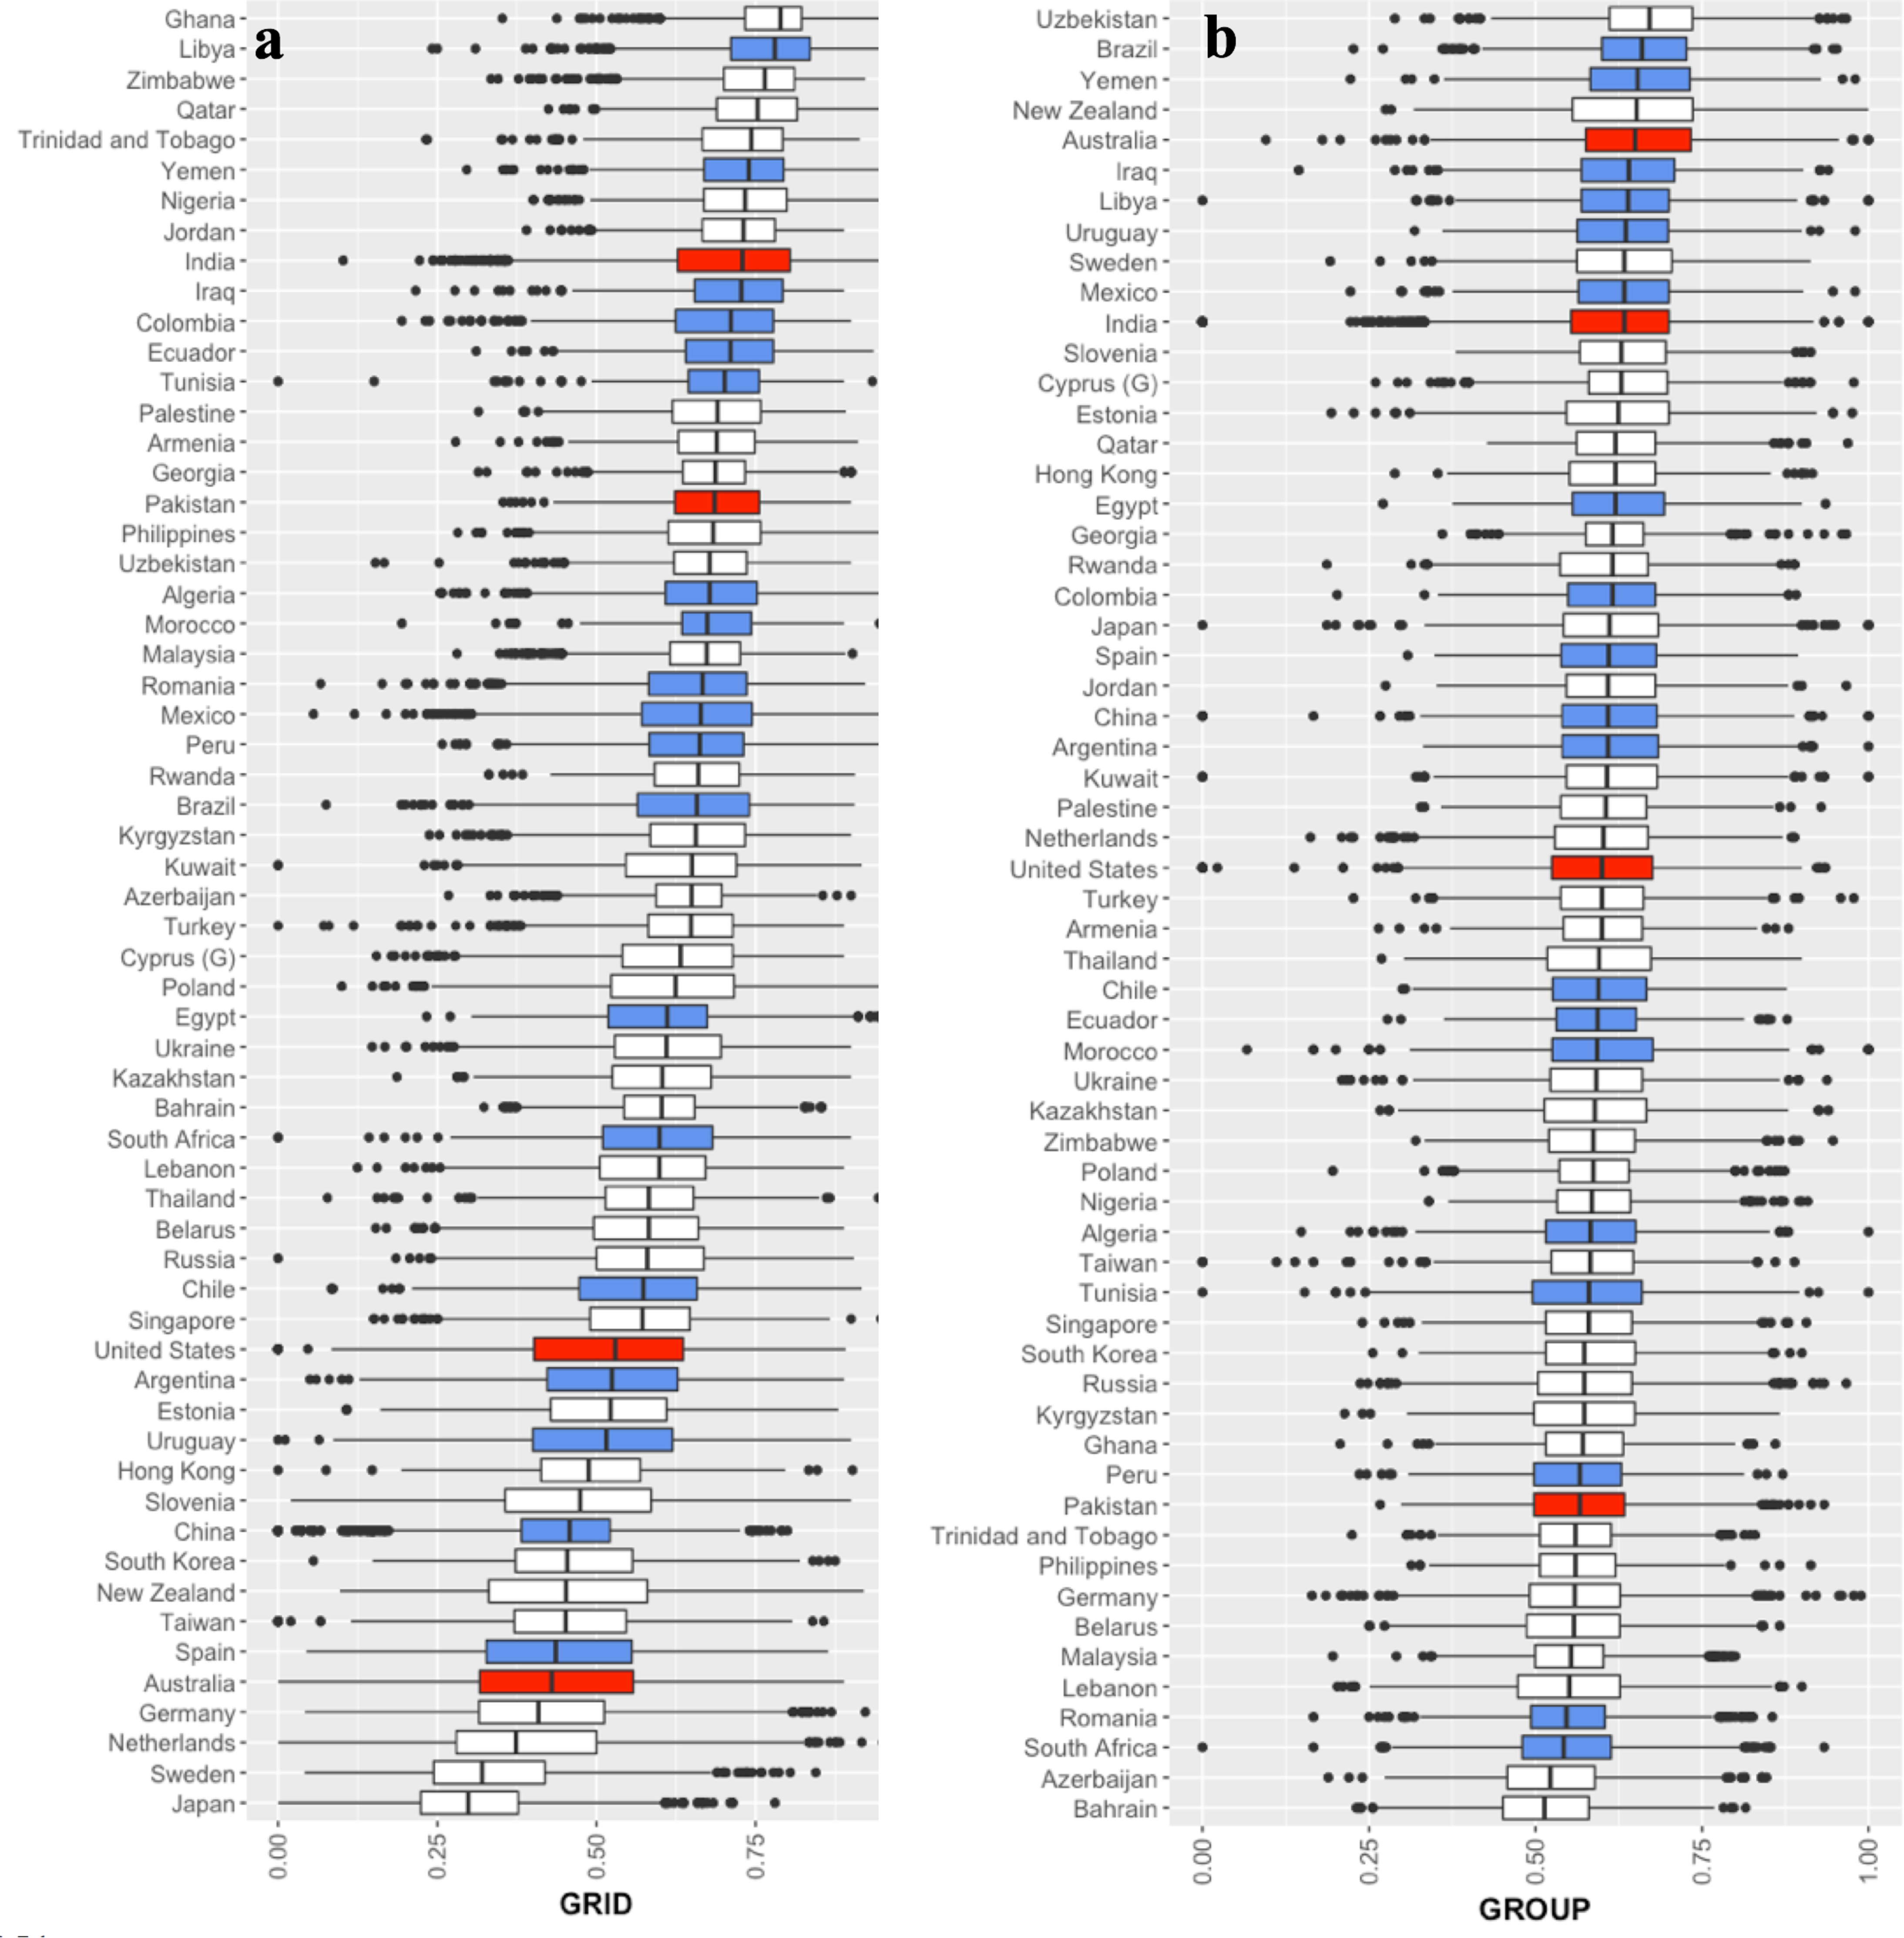
\includegraphics[width=0.8\paperwidth]{Figures/CH3_Methods_Fig1}}
	\end{center}
\end{figure}

\begin{figure}
	\caption{Effect of increasing monitoring and enforcement powers (M,F). Columns correspond to our three case studies, ordered from left to right according to increasing group size (see Supplementary Figure \ref{fig: CH3_GCG1_Representative group sizes}). Rows show increasing enforcement powers (M=monitoring; F=fines). Shaded boxes show grid and group interquartile ranges obtained from the World Values Survey Wave 6. Contours indicate the percentage of agents that comply with groundwater conservation policies. Insets show ensemble standard deviations of 100 independent realisations. } \label{fig: CH3_GCG1_WVS raw statistics}
	\begin{center}
	\makebox[\textwidth]{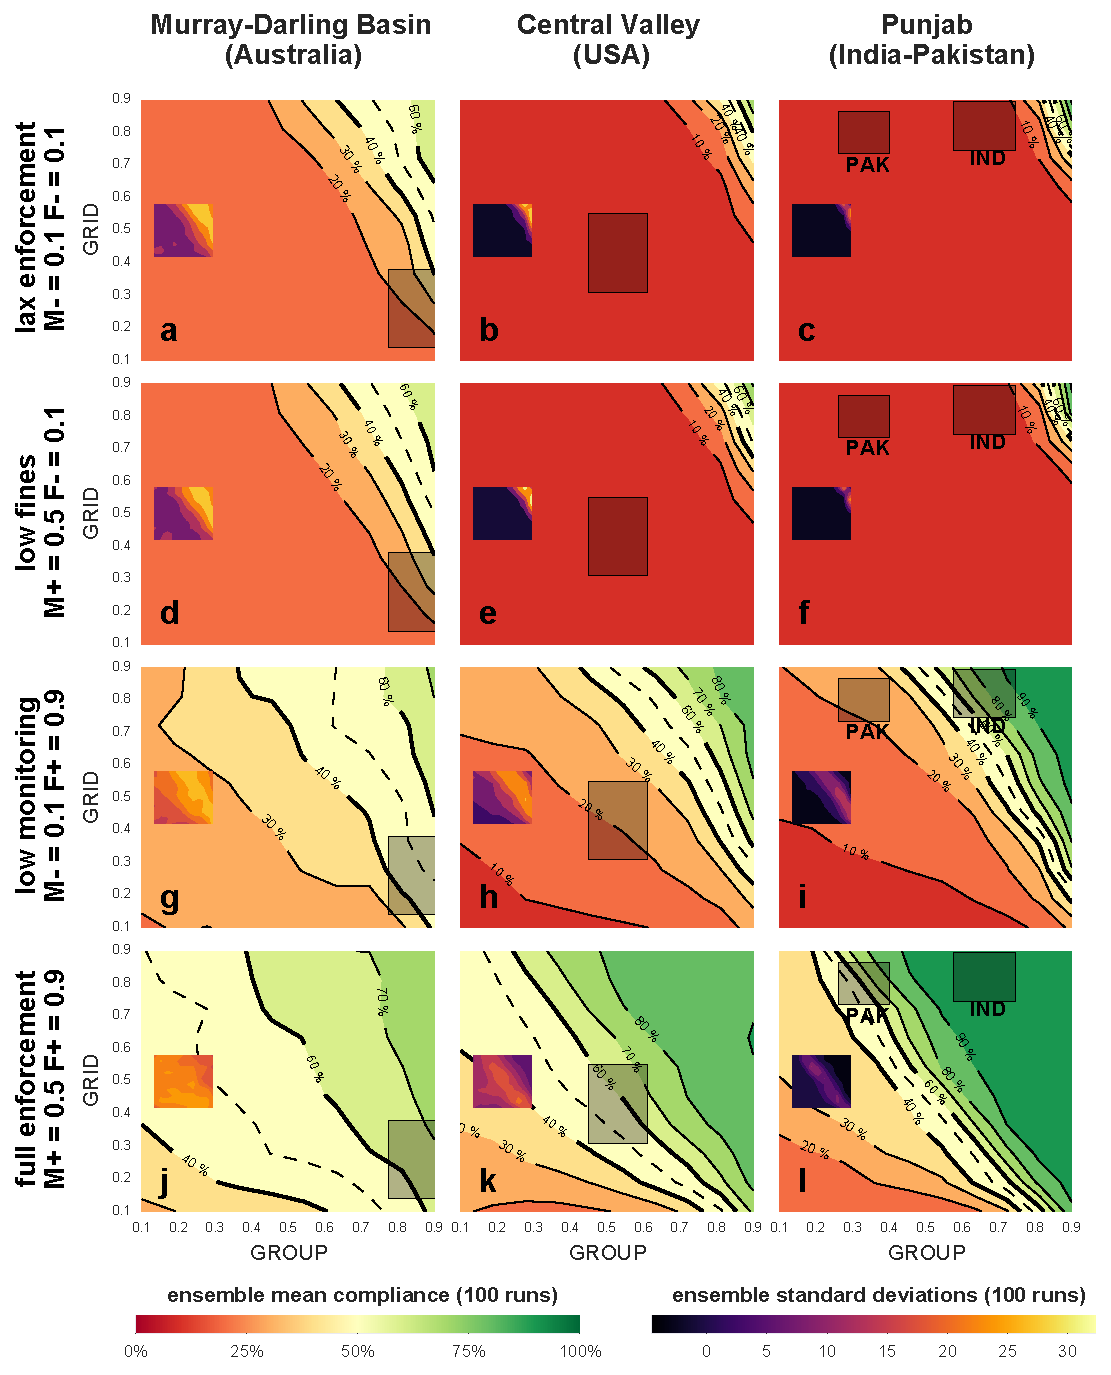
\includegraphics[width=0.7\paperwidth]{Figures/CH3_Methods_Fig2}}
	\end{center}
\end{figure}

\begin{figure} \caption{Representative group sizes for countries with aquifers of national and transboundary importance. (a) average land holdings computed from FAOSTAT (\url{http://www.fao.org/faostat/}). (b) GCG implementation of group size effects. Top panels show typical spatial distributions of land holdings in a 10x10 [km] region from Google Earth Imagery. Bottom panels show corresponding agent-based representations. See Supplementary Data Table 1 for agro-economic data used to parametrise GCG simulations in each case. Dots represent individual farmers while cells represent the computational discretisation.} \label{fig: CH3_GCG1_Representative group sizes}  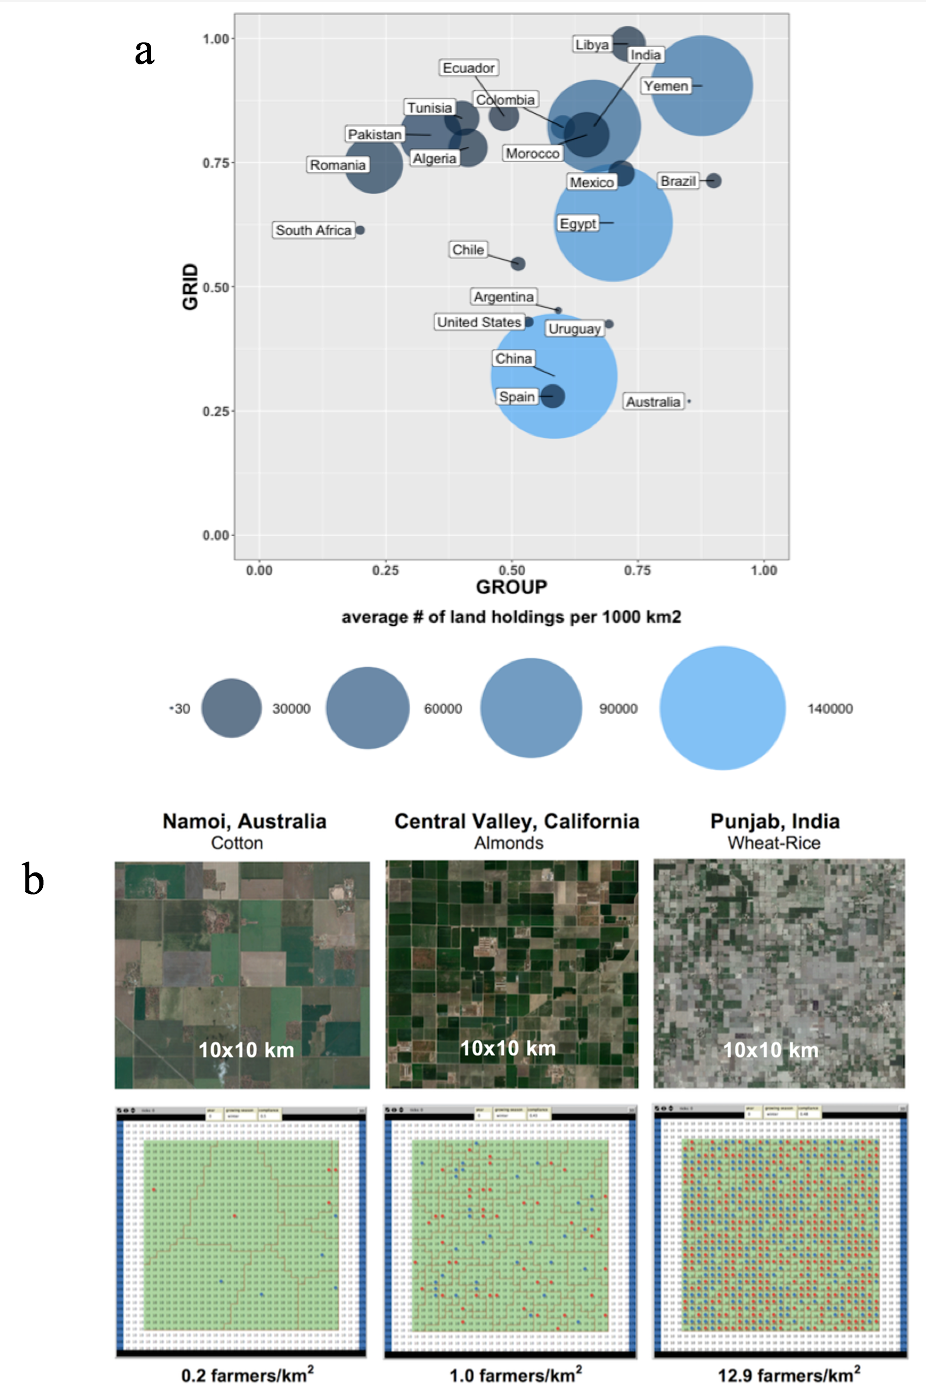
\includegraphics[width=0.9\textwidth]{Figures/CH3_Methods_Fig3} \end{figure} 

\begin{figure}
	\caption{Grid-Group positions and compliance revealed by our Murray-Darling Basin surveys \autocite{Holley:2015te} are consistent with WVS6 statistics and GCG simulations. (a) grid and group statistics from the WVS6 did not differ significantly (parametric two sample t-test; P=0.12 for grid and P=0.65 for group) from scores computed from our surveys in eastern Australia. (b) comparison of observed (our survey) and GCG-simulated compliance. Black contours indicate GCG outputs across M-F space. Solid blue lines indicate interquartile range, and the dashed line the mean from our surveys. Shaded box shows interquartile range for M and F obtained from our surveys.} \label{fig: CH3_GCG1_WVS-MDB validation}
	\begin{center}
	\makebox[\textwidth]{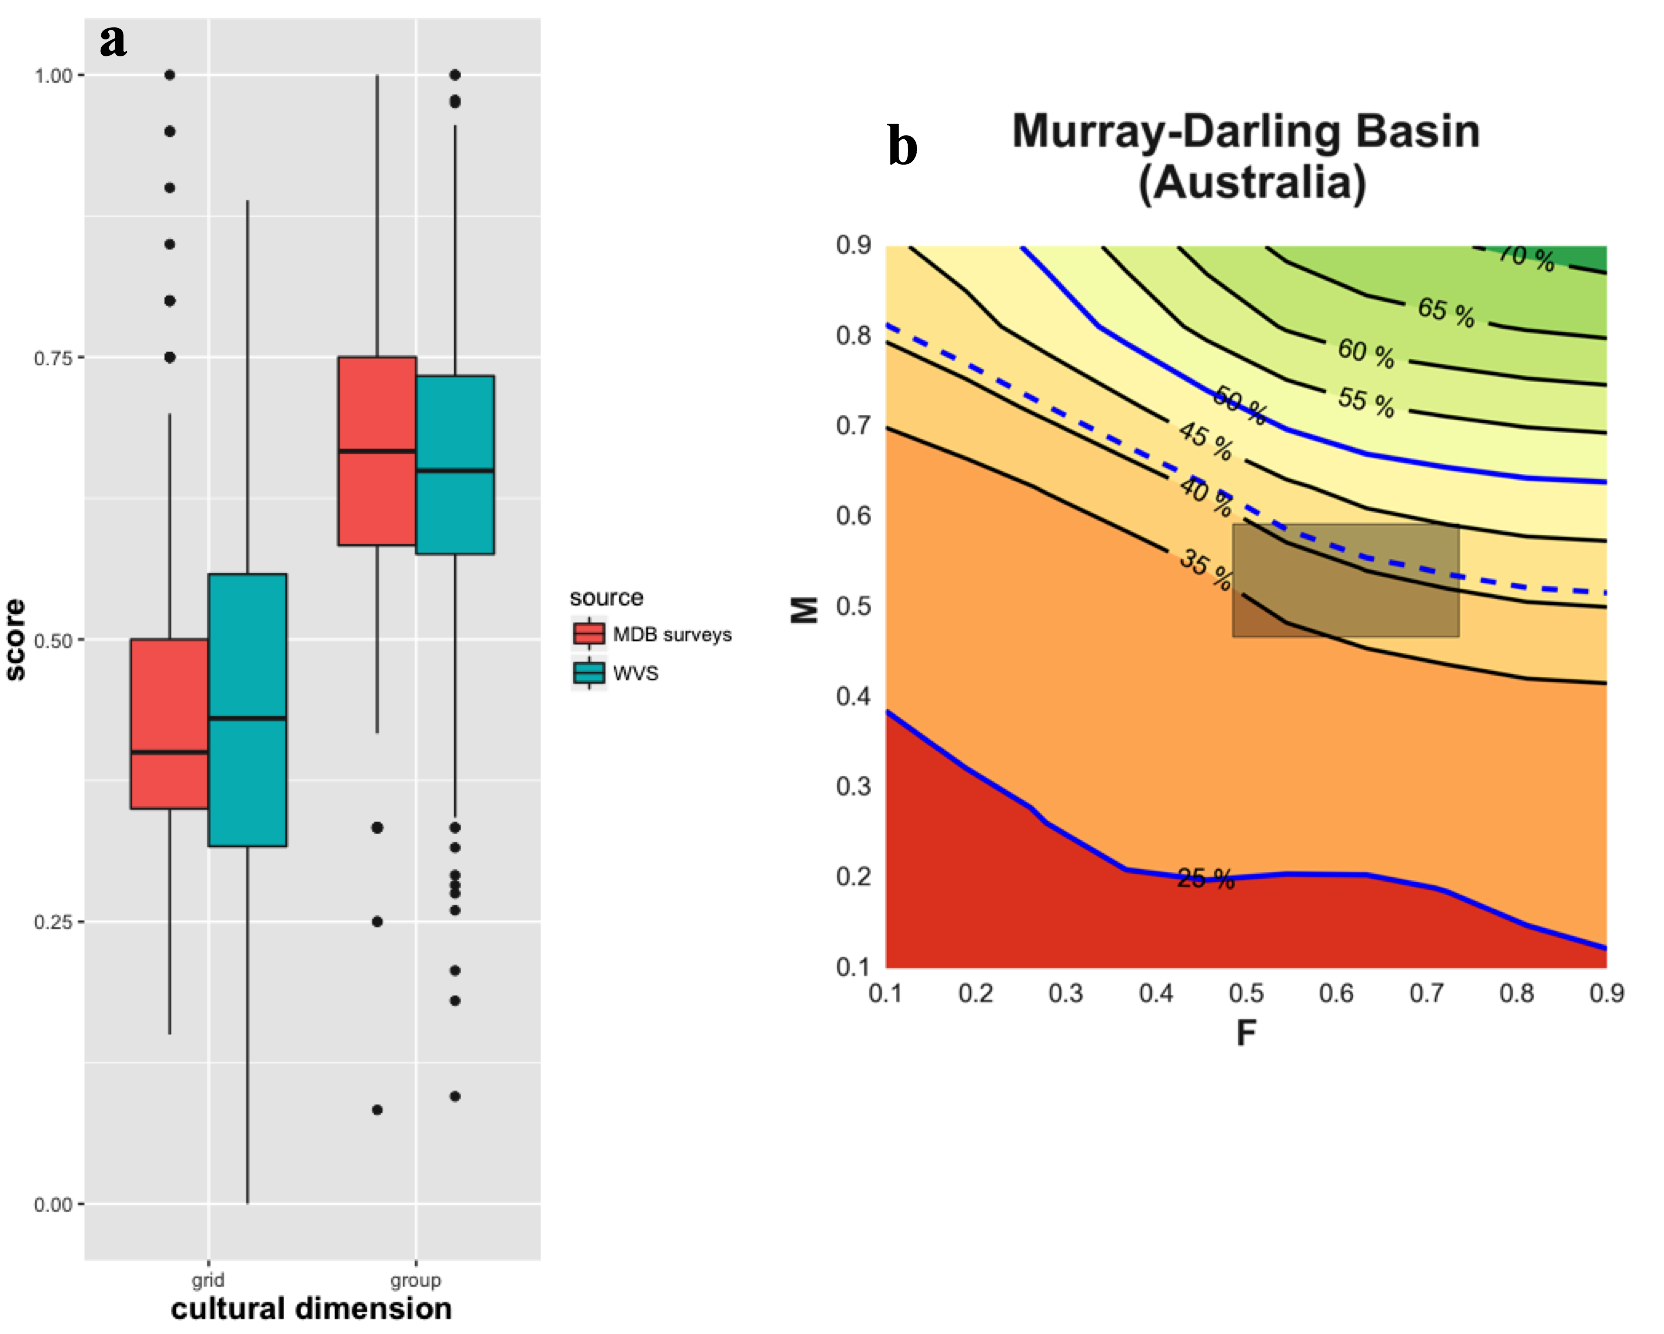
\includegraphics[width=0.8\paperwidth]{Figures/CH3_Methods_Fig4}}
	\end{center}
\end{figure} 

\begin{figure}
	\caption{GCG main processes. (top) schematic of agent dynamics (bottom) scheduling of agent and groundwater processes.}\label{Fig: CH3_GCG1_Flow diagram agent processes}
	\begin{center}
	\makebox[\textwidth]{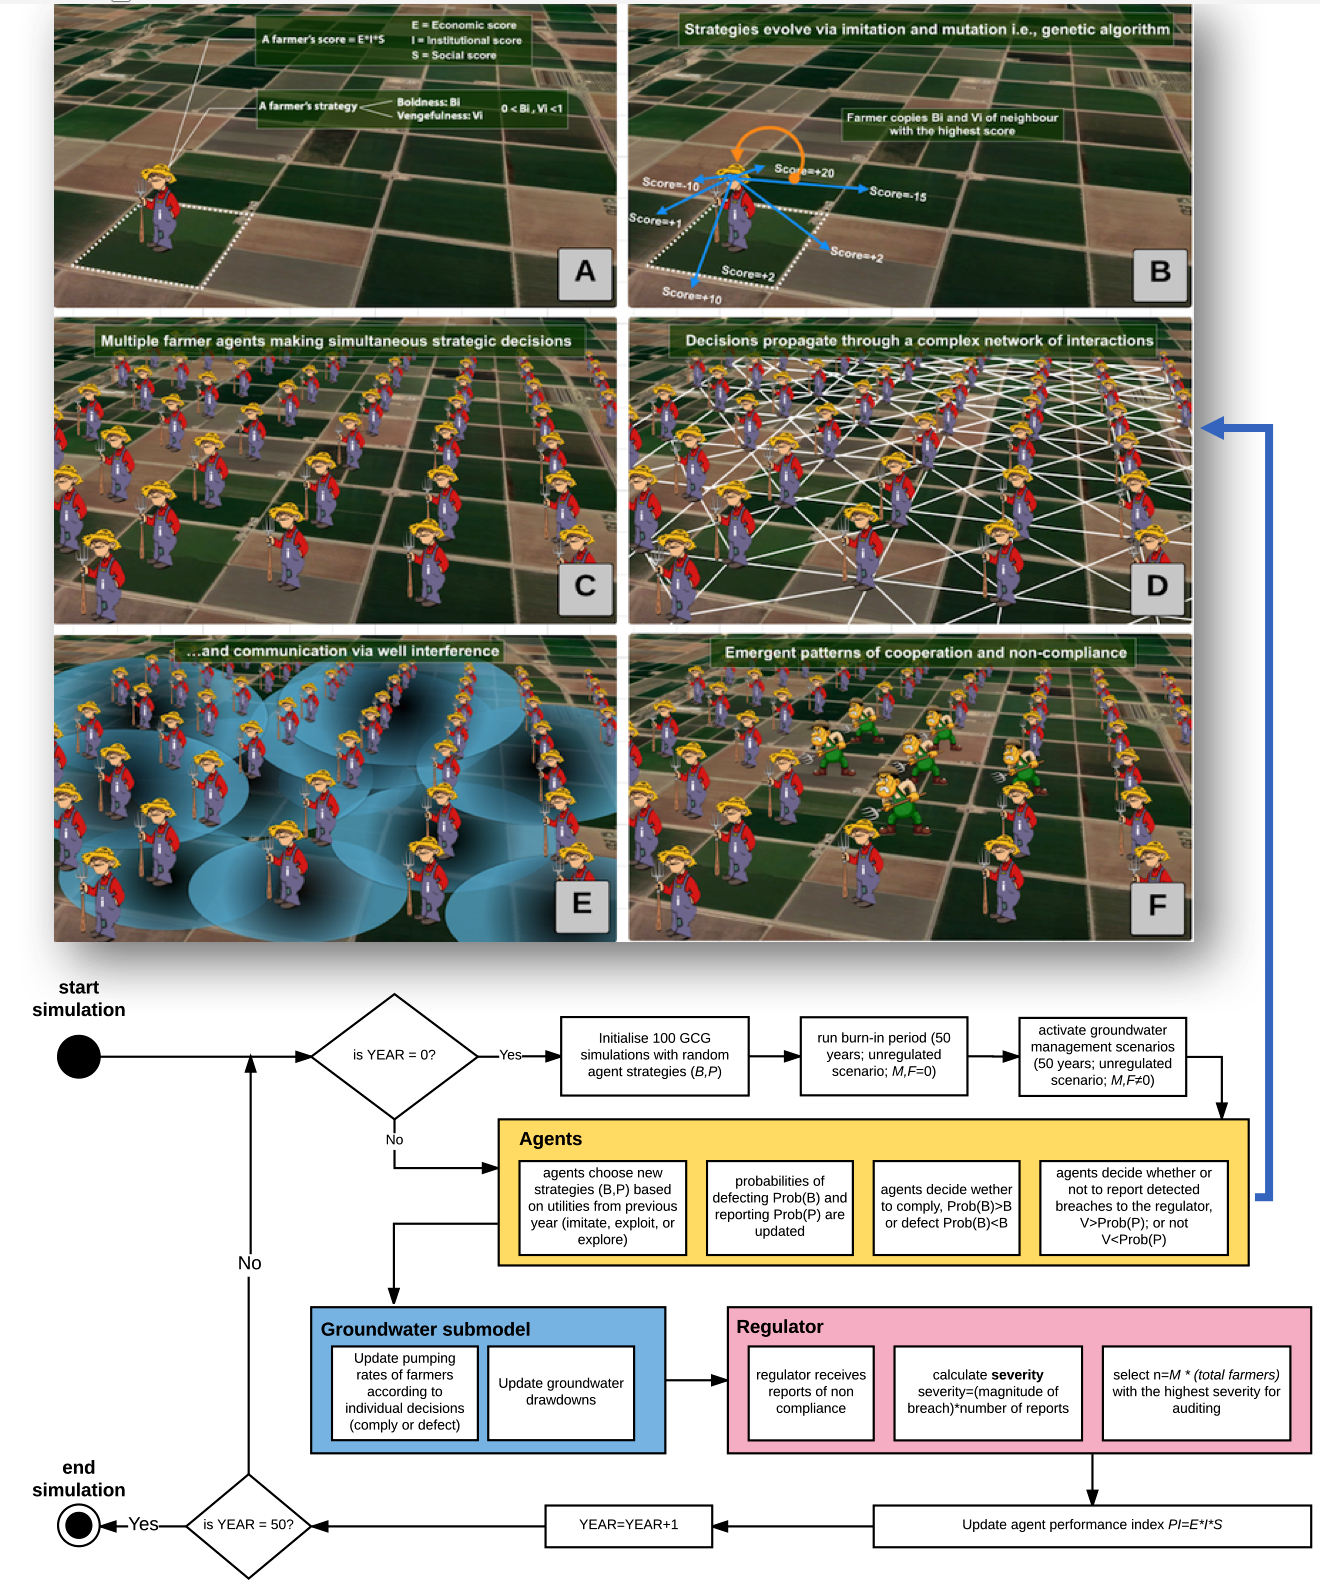
\includegraphics[width=0.8\paperwidth]{Figures/CH3_ODD_Fig1}}

	\end{center}
\end{figure}

\begin{sidewaysfigure}
	\caption{Agent-based implementation of the GCG in FlowLogo. User interface for one of our case studies. Model window shows time series and histograms coupled social-groundwater output; sliders and switches to set base parameters for agents; controls for cultural variables and policy intervention mechanisms.} \label{fig: CH3_GCG1_Implementation of the GCG in FlowLogo}
	\begin{center}
	\makebox[\textwidth]{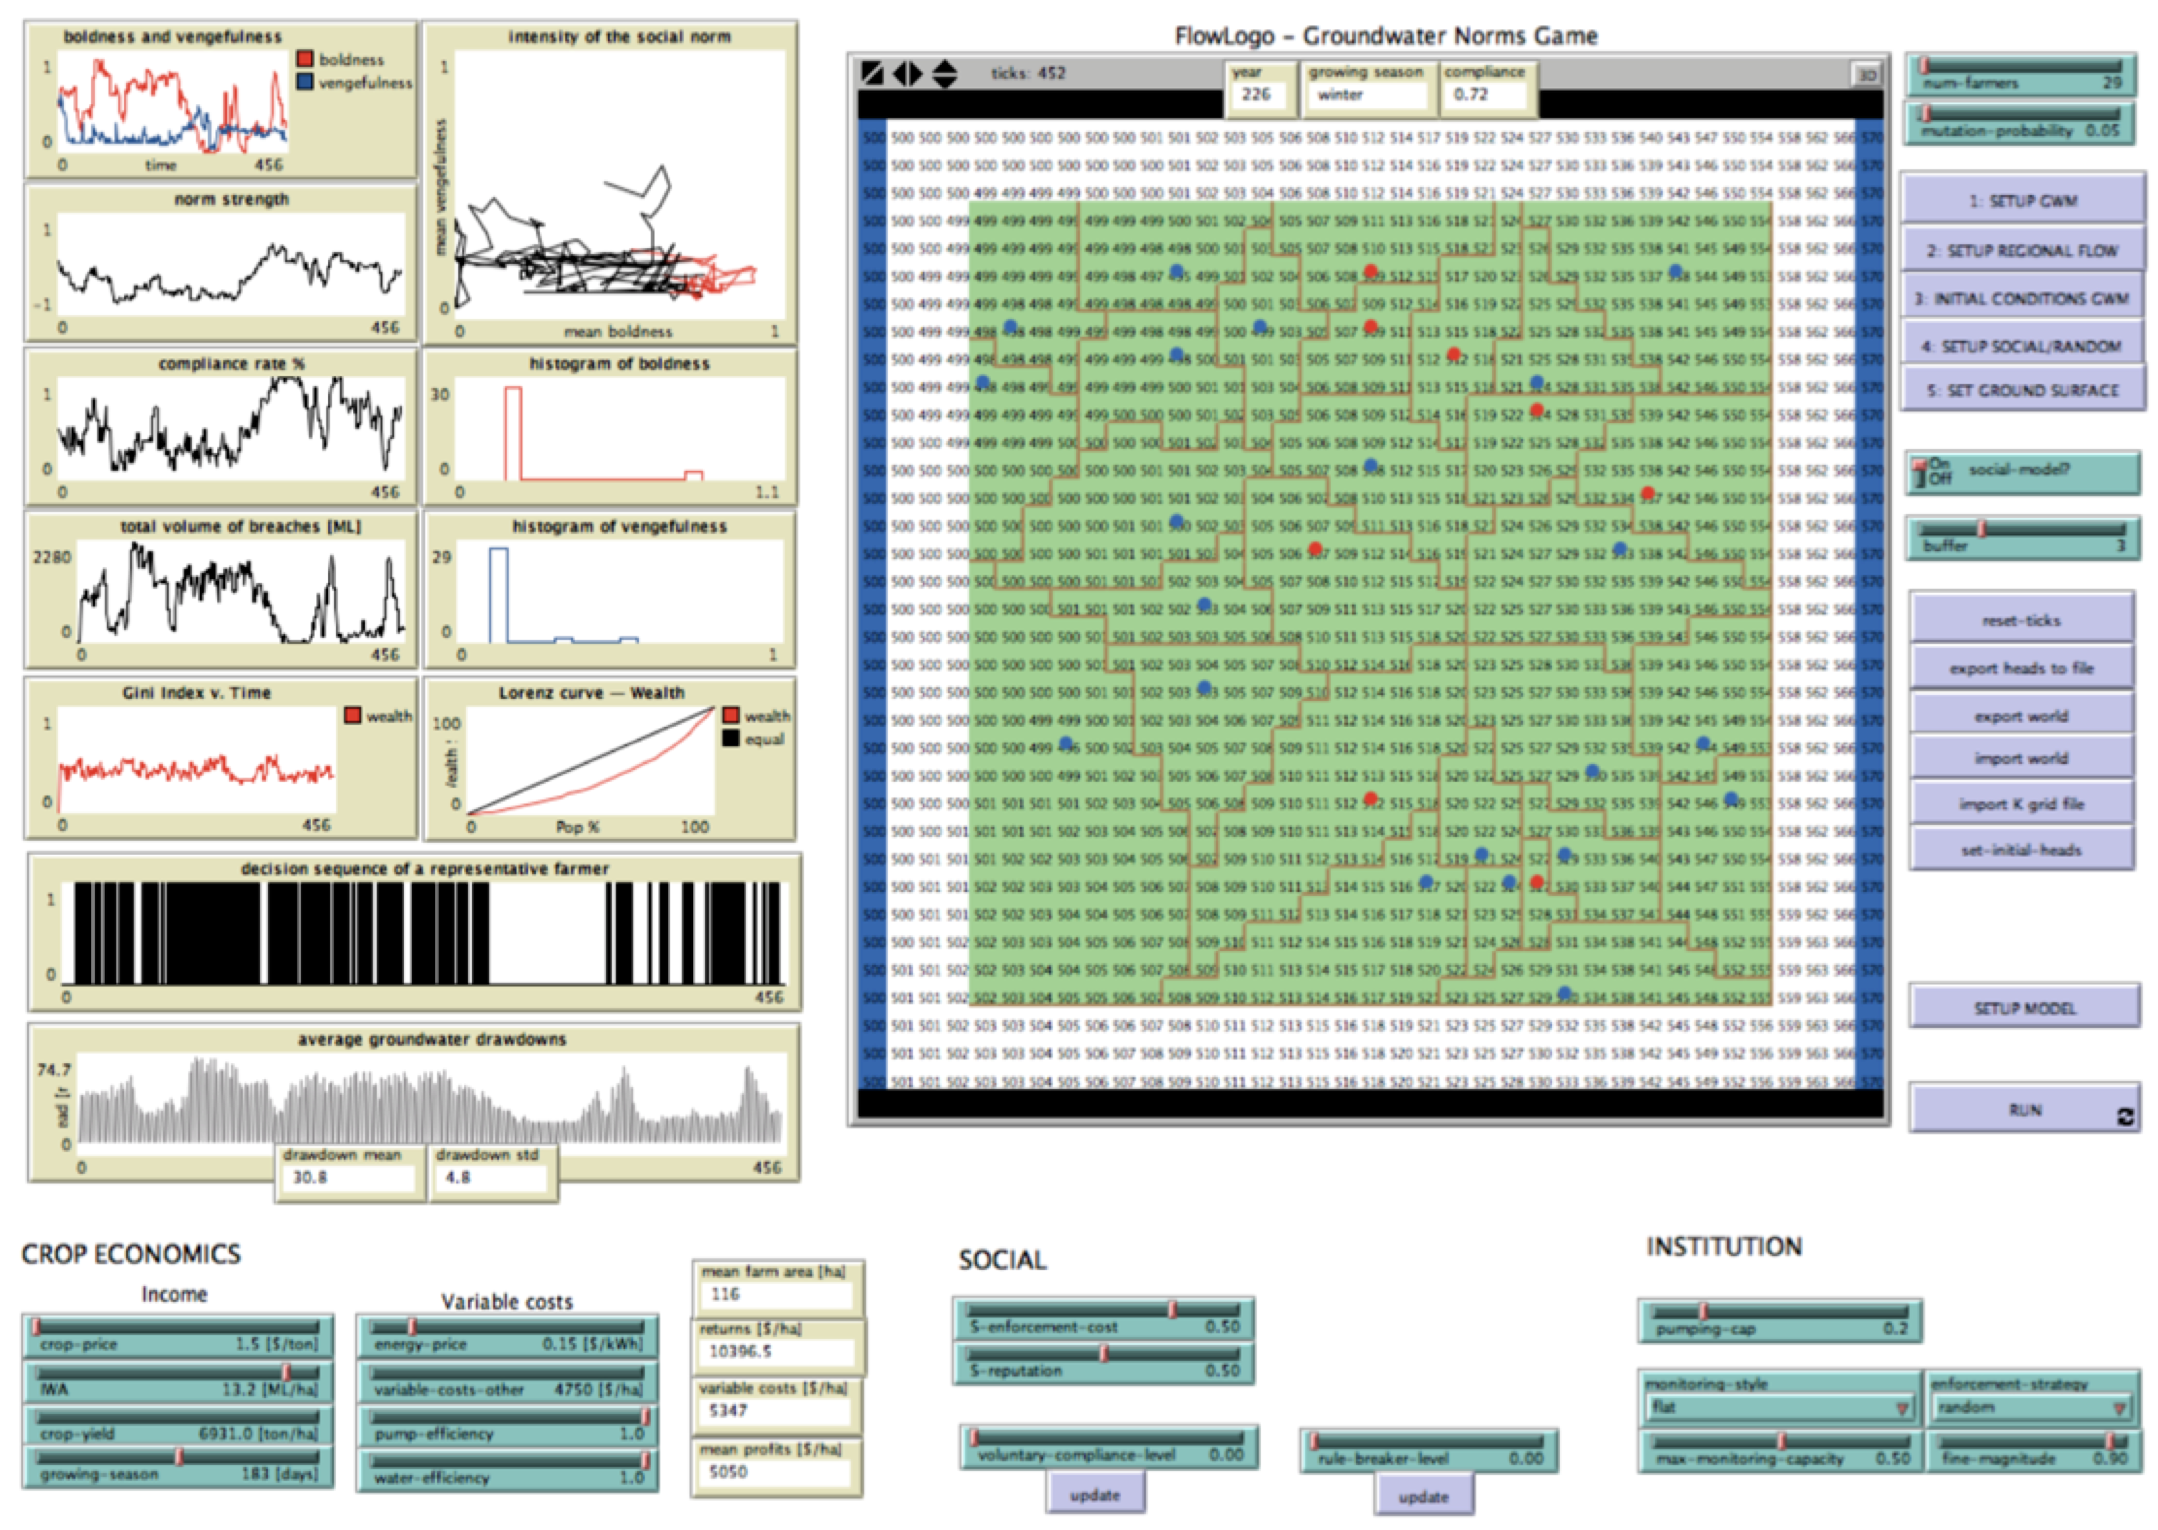
\includegraphics[width=0.8\paperwidth]{Figures/CH3_ODD_Fig2}}
	\end{center}
\end{sidewaysfigure}

\begin{figure}
	\caption{Socio-economic dynamics in the GCG represented as ‘forces’ pulling agent decisions in opposite directions.}  \label{fig: CH3_GCG1_Socio-economic dynamics "forces"} 
	\begin{center}
	\makebox[\textwidth]{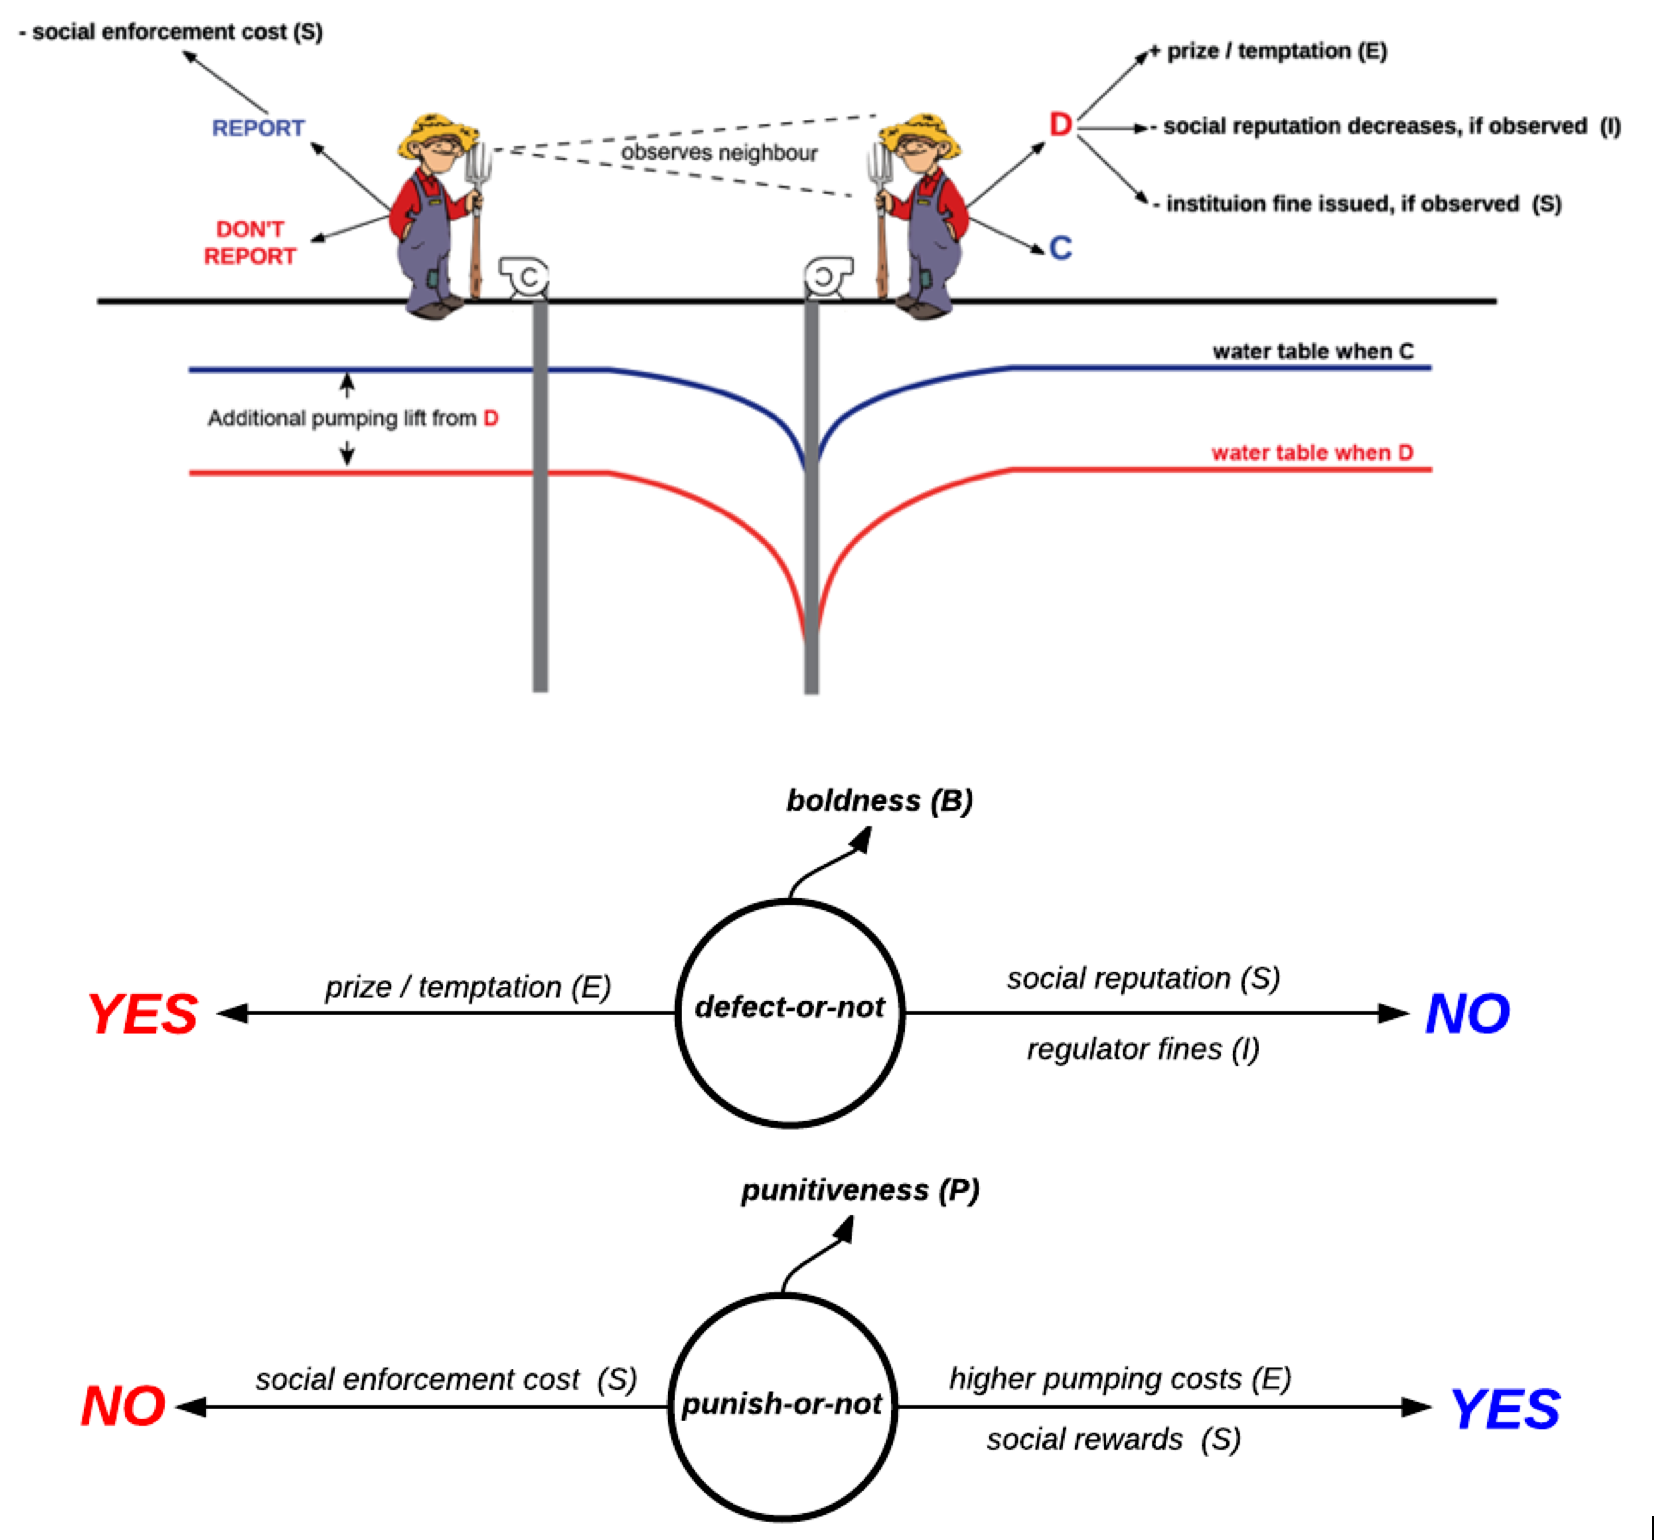
\includegraphics[width=0.8\paperwidth]{Figures/CH3_ODD_Fig3}}
	\end{center}
\end{figure}

\begin{figure}
	\caption{Functional form of the social utility function of agents in the GCG.}
	\label{Fig: CH3_GCG1_Social utility function}
	\begin{center}
	\makebox[\textwidth]{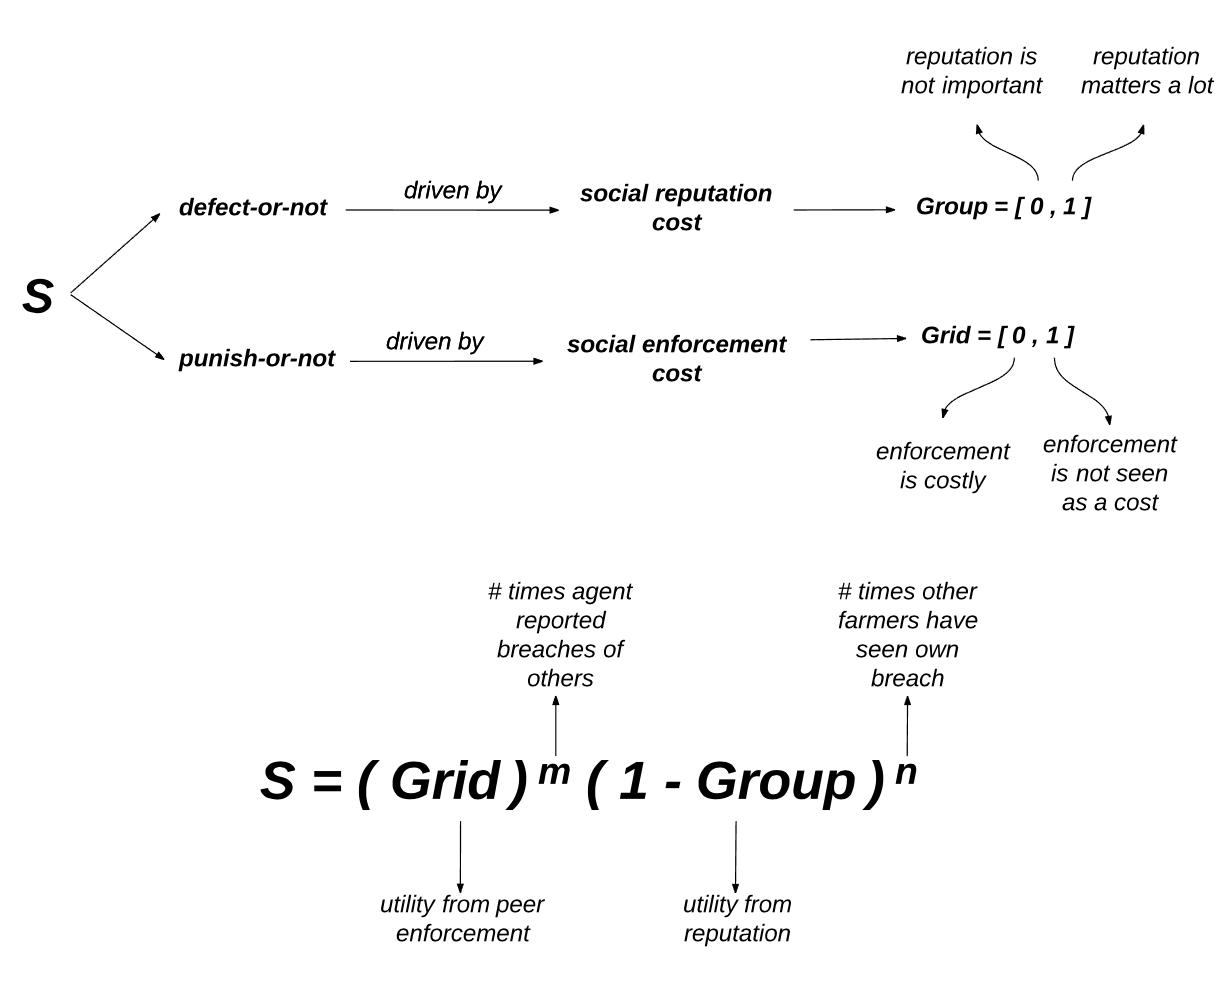
\includegraphics[width=0.8\paperwidth]{Figures/CH3_ODD_Fig4}}
	\end{center}
\end{figure}

\begin{figure}
	\caption{Schematic of compliance and enforcement strategies of a typical water authority 
	\autocite{Holley:2012tg,Ayres:1992vm,Braithwaite:2012wb} and functional form of the institutional utility function of agents in the GCG.} 	\label{Fig: CH3_GCG1_Institutional utility function} 
	\begin{center}
	\makebox[\textwidth]{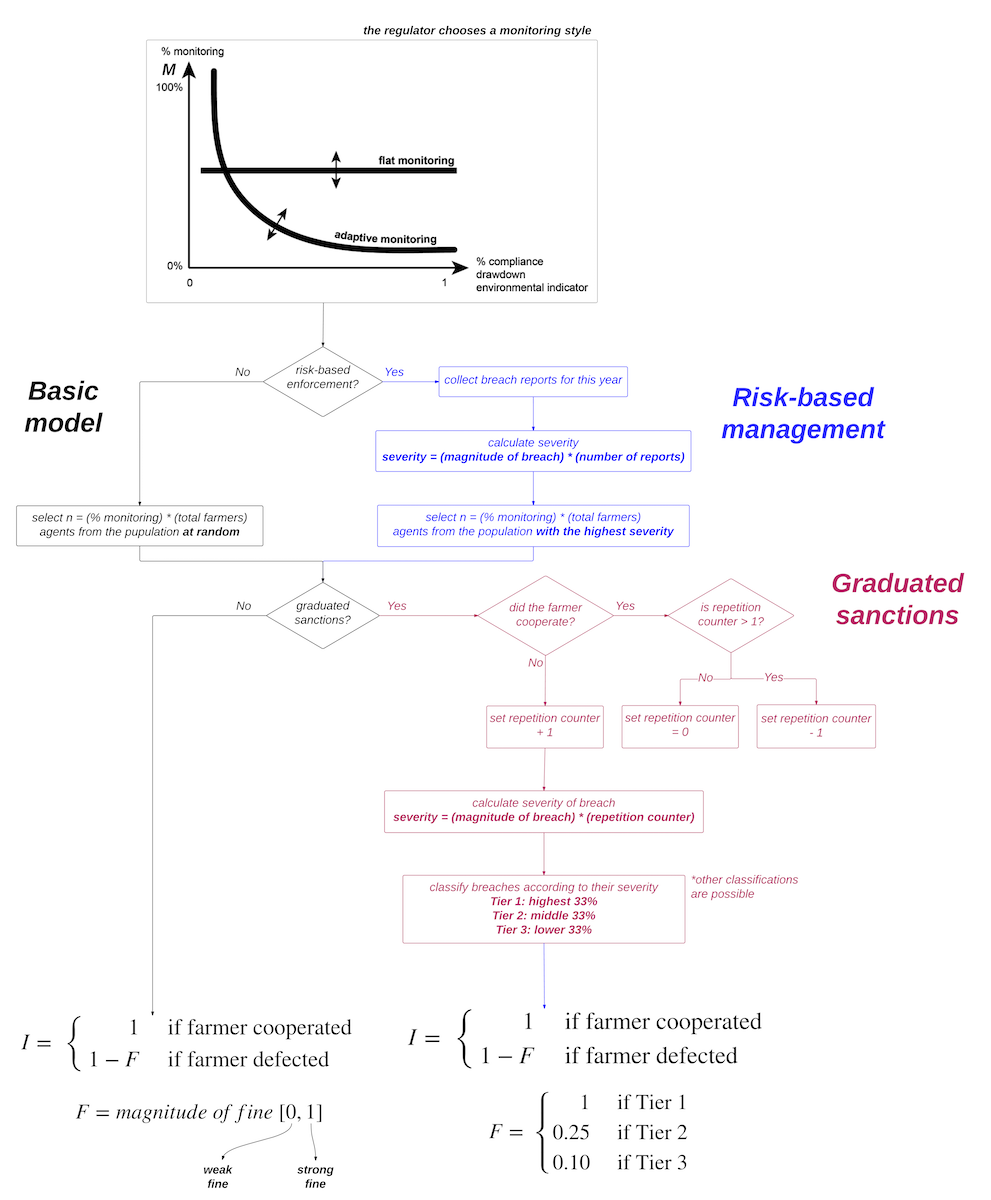
\includegraphics[width=0.8\paperwidth]{Figures/CH3_ODD_Fig5}}
	\end{center}
\end{figure}

\begin{figure}
	\caption{Functional form of the economic utility function of agents in the GCG.}
	\label{Fig: CH3_GCG1_Economic utility function} 
	\begin{center}
	\makebox[\textwidth]{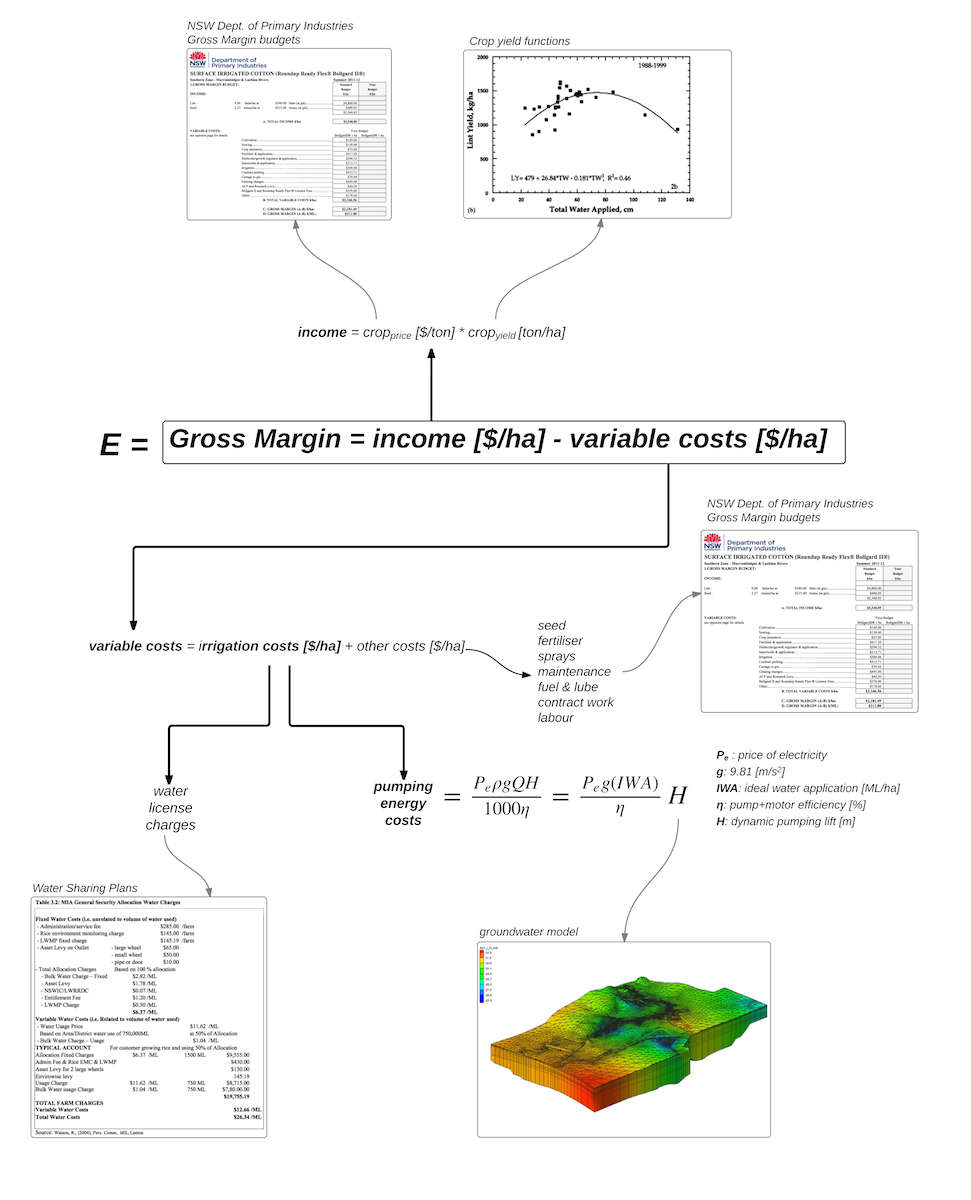
\includegraphics[width=0.8\paperwidth]{Figures/CH3_ODD_Fig6}}
	\end{center}
\end{figure}

%%%%%%%%%%%%%%%%%%%%%%%%%%%%%%%%%%%%%%
%%%%%%% SUPPLEMENTARY TABLES %%%%%%%%%
%%%%%%%%%%%%%%%%%%%%%%%%%%%%%%%%%%%%%%

\begin{sidewaystable}
\caption{Grid-Group categories and one-way analysis of variance (ANOVA) for the World Values Survey Wave 6}
\label{table: WVS grid-group questions}
\begin{adjustbox}{width=\textwidth}
\begin{tabular}[]{p{0.1\textwidth}lp{0.1\textwidth}p{0.35\textwidth}lllll}
\toprule
\textbf{Cultural dimension} &
\textbf{Variable} & 
\textbf{question code} & 
\textbf{Value orientation
question} & 
\textbf{High } & 
\textbf{Low} & 
\textbf{Mean} & 
\textbf{SD} & \textbf{F-value*}
\tabularnewline
\midrule
\textbf{GRID} & \textbf{Grid 1} & V9 & \emph{Religion} & Important & Not
important & 0.71 & 0.35 & 820.7\tabularnewline
& \textbf{Grid 2} & V164 & \emph{Job old/young} & Old acceptable & Old
unacceptable & 0.44 & 0.30 & 44.8\tabularnewline
& \textbf{Grid 3} & V21 & \emph{Follow instructions} & Yes & Not
necessary & 0.41 & 0.49 & 79.3\tabularnewline
& \textbf{Grid 4} & V69 & \emph{Respect authority} & Yes & No & 0.74 &
0.35 & 402.4\tabularnewline
& \textbf{Grid 5} & V152 & \emph{Religion (God)} & God important & Not
important & 0.75 & 0.33 & 114.5\tabularnewline
& \textbf{Grid 6} & V203 & \emph{Justifiable: homosexuality} & Never
justifiable & Justifiable & 0.75 & 0.34 & 52.8\tabularnewline
& \textbf{Grid 7} & V203A & \emph{Justifiable: prostitution} & Never
justifiable & Justifiable & 0.80 & 0.28 & 69.2\tabularnewline
& \textbf{Grid 8} & V204 & \emph{Justifiable: abortion} & Never
justifiable & Justifiable & 0.75 & 0.31 & 337.3\tabularnewline
& \textbf{Grid 9} & V200 & \emph{Justifiable: stealing property} & Never
justifiable & Justifiable & 0.09 & 0.20 & 403.6\tabularnewline
& \textbf{Grid 10} & V77 & \emph{Behave properly; avoid doing anything
people would say is wrong} & Very much like me & Not at all like me &
0.69 & 0.27 & 179.6\tabularnewline
& \textbf{~} & ~ & ~ & ~ & ~ & ~ & ~ & ~\tabularnewline
\textbf{GROUP} & \textbf{Group 1} & V4 & \emph{Importance: Family} &
Important & Not important & 0.97 & 0.12 & 428.1\tabularnewline
& \textbf{Group 2} & V5 & \emph{Importance: Friends} & Important & Not
important & 0.77 & 0.25 & 46.2\tabularnewline
& \textbf{Group 3} & V24 & \emph{Trust people} & Most can be trusted &
Have to be careful & 0.25 & 0.43 & 53.5\tabularnewline
& \textbf{Group 4} & V71 & \emph{Importance: money} & Less emphasis &
More emphasis & 0.55 & 0.31 & 110.1\tabularnewline
& \textbf{Group 5} & V98 & \emph{Responsibility: personal/government} &
Government & Personal & 0.61 & 0.32 & 85.5\tabularnewline
& \textbf{Group 6} & V20 & \emph{Being unselfish} & Mentioned & Not
mentioned & 0.34 & 0.47 & 105.4\tabularnewline
& \textbf{Group 7} & V74 & \emph{Doing something for society} & Very
much like me & Not at all like me & 0.70 & 0.25 & 26.6\tabularnewline
& \textbf{Group 8} & V78 & \emph{Looking after the environment} & Very
much like me & Not at all like me & 0.70 & 0.26 & 50.0\tabularnewline
& \textbf{Group 9} & V216 & \emph{I see myself as an autonomous
individual} & Strongly disagree & Strongly agree & 0.36 & 0.32 &
104.8\tabularnewline
& \textbf{Group 10} & V213 & \emph{I see myself as part of my local
community} & Strongly agree & Strongly disagree & 0.74 & 0.27 &
260.4\tabularnewline
\bottomrule
\end{tabular}
\end{adjustbox}
\\
\footnotesize{*All the between-country F-values are significant at P<0.001}
\end{sidewaystable}


\begin{sidewaystable}[]
\caption{Grid-Group categories and indexes for our Murray-Darling Basin surveys} \label{table: MDB grid-group questions}
\begin{adjustbox}{width=\textwidth}
\begin{tabular}[]{p{0.1\textwidth}lp{0.3\textwidth}p{0.07\textwidth}p{0.07\textwidth}p{0.05\textwidth}p{0.07\textwidth}p{0.07\textwidth}p{0.07\textwidth}p{0.1\textwidth}p{0.1\textwidth}p{0.07\textwidth}}
\toprule
\textbf{Cultural dimension} &
\textbf{Variable} & \textbf{Value orientation question} & \textbf{High }
& \textbf{Low} & \textbf{Table \autocite{Holley:2015te}} & \textbf{question code} &
\textbf{question mapping} & \textbf{survey score} & \textbf{normalised
score} & \textbf{question score} & \textbf{GCG score}\tabularnewline
\midrule
\textbf{GRID} & \textbf{Grid 1} & \emph{Complying with water laws is the
right thing to do} & Strongly agree & Strongly disagree & 4.1 & q3law &
Grid + & 4.28 & 0.82 & 0.82 & \textbf{0.433}\tabularnewline
& \textbf{Grid 2} & \emph{Water regulation is needed to sustainably
manage water resources} & Strongly disagree & Strongly agree & 4.2 &
q1sus & Grid - & 4.16 & 0.79 & 0.21 &\tabularnewline
& \textbf{Grid 3} & \emph{Water regulation is needed to protect the
rights of water users} & Strongly disagree & Strongly agree & 4.2 &
q1pro & Grid - & 4.14 & 0.79 & 0.22 &\tabularnewline
& \textbf{Grid 4} & \emph{Water regulation is needed to protect the
long-term viability of communities} & Strongly disagree & Strongly agree
& 4.2 & q1com & Grid - & 4.20 & 0.80 & 0.20 &\tabularnewline
& \textbf{Grid 5} & \emph{Justifiable: illegal taking of water under
tough economic conditions} & Strongly disagree & Strongly agree & 4.4 &
q3ill & Grid - & 2.13 & 0.28 & 0.72 &\tabularnewline
\textbf{~} & \textbf{~} & \emph{~} & ~ & ~ & ~ & ~ & ~ & ~ & ~ & ~ &
\textbf{~}\tabularnewline
\textbf{GROUP} & \textbf{Group 1} & \emph{Complying with my licence
conditions is important because breaking the rules is unfair to other
water users} & Strongly agree & Strongly disagree & 4.1 & q3lic & Group
+ & 4.23 & 0.81 & 0.81 & \textbf{0.657}\tabularnewline
& \textbf{Group 2} & \emph{Complying with my licence conditions is
important because breaking the rules reflects badly on my reputation
with my peers} & Strongly disagree & Strongly agree & 4.1 & q3rep &
Group + & 4.02 & 0.76 & 0.76 &\tabularnewline
& \textbf{Group 3} & \emph{Getting a criminal record for carrying out
illegal water activities is a strong deterrent } & Strongly agree &
Strongly disagree & 4.3 & q3crim & Group + & 3.65 & 0.66 & 0.66
&\tabularnewline
& \textbf{Group 4} & \emph{Illegal water extraction occurs because of a
desire for economic advantage} & Strongly disagree & Strongly agree &
4.4 & q3econ & Group - & 3.39 & 0.60 & 0.40 &\tabularnewline
\bottomrule
\end{tabular}
\end{adjustbox}	
\end{sidewaystable}

\begin{sidewaystable}
\caption{Agro-economic data for the three case studies.} \label{table: GCG agro-economic data}
\begin{adjustbox}{width=\textwidth}	
\begin{tabular}[]{lp{0.25\textwidth}p{0.07\textwidth}p{0.1\textwidth}p{0.07\textwidth}lp{0.07\textwidth}lll}
\toprule
& & \multicolumn{2}{l}{\textbf{Australia}} & \multicolumn{2}{l}{\textbf{United States}} & \multicolumn{4}{l}{\textbf{India-Pakistan}} \tabularnewline
\midrule
& & & & & & & & &\tabularnewline
& \textbf{Representative region} & \multicolumn{2}{l}{\textbf{Murray-Darling}†} & \multicolumn{2}{l}{\textbf{Central Valley‡}} & \multicolumn{4}{l}{\textbf{Punjab Basin§}}\tabularnewline
& & & & & & & & &\tabularnewline
& \textbf{Crop} & Cotton & & Almonds & & Rice & & Wheat
&\tabularnewline
& \textbf{Average farm size} & 362 & ha & 74 & ha & 4 & ha & 4 &
ha\tabularnewline
& \textbf{Yield} & 10.5 & bales/ha & 6930.7 & lb/ha & 6960.0 & kg/ha &
5525.0 & kg/ha\tabularnewline
& \textbf{Price} & 580 & AUD/bale & 1.5 & USD/lb & 0.11 & USD/kg & 0.12
& USD/kg\tabularnewline
\textbf{A} & \textbf{Revenue} & 6090 & AUD/ha & 10396 & USD/ha & 766 &
USD/ha & 663 & USD/ha\tabularnewline
& & & & & & & & &\tabularnewline
& \textbf{Total costs} & 3395 & AUD/ha & 6101 & USD/ha & 411 & USD/ha &
216 & USD/ha\tabularnewline
& \textbf{Costs of irrigation} & 570 & AUD/ha & 1351 & USD/ha & 89 &
USD/ha & 27 & USD/ha\tabularnewline
& \textbf{Irrigation water requirement} & 9.5 & ML/ha & 13.2 & ML/ha &
13.52 & ML/ha & 4.1 & ML/ha\tabularnewline
& \textbf{Electricity price} & 0.20 & AUD/kWh & 0.15 & USD/kWh & 0.016 &
USD/kWh & 0.016 & USD/kWh\tabularnewline
\textbf{B} & \textbf{Total costs minus irrigation} & 2825 & AUD/ha &
4750 & USD/ha & 322 & USD/ha & 189 & USD/ha\tabularnewline
& & & & & & & & &\tabularnewline
\textbf{A - B} & \textbf{Gross margin* } & 3265 & AUD/ha & 5646 & USD/ha
& 444 & USD/ha & 474 & USD/ha\tabularnewline
\bottomrule
\end{tabular}
\end{adjustbox}
\\
\footnotesize{*gross margins do not include pumping electricity costs \\(included at runtime during simulations, based on drawdowns obtained from the groundwater sub-model)}
\\
\footnotesize{†2015 Australian Cotton Production Manual; \url{http://www.cottoninfo.com.au/publications}}
\\
\footnotesize{‡UC Davis Agricultural and Crop Economics, \url{http://coststudies.ucdavis.edu}}
\\
\footnotesize{§ see \autocite{Jalota:2007ha,Singh:2009jo}}
\end{sidewaystable}

%%%%%%%%%%%%%%%%%%%%%%%%%%%%%%%%%%%%%%%%%
%%%%%%% SUPPLEMENTARY REFERENCES %%%%%%%%
%%%%%%%%%%%%%%%%%%%%%%%%%%%%%%%%%%%%%%%%%
\FloatBarrier

\addcontentsline{toc}{section}{Supplementary References}

\printbibliography[title={Supplementary References}]

\end{document}
